\chapter{AdaptativeSR: pruning-based Topology Refinement of 3D Mesh using a 2D Alpha Mask
}
\label{chapter:appendix-adaptativeSR}

%\minitoc
\chapterwithfigures{\nameref*{chapter:appendix-adaptativesr}}
\chapterwithtables{\nameref*{chapter:appendix-adaptativesr}}

\ifthenelse{\boolean{skipAppendix}}{\endinput}{}


Image-based 3D reconstruction has increasingly stunning results over the past few years with the latest improvements in computer vision and graphics. Geometry and topology are two fundamental concepts when dealing with 3D mesh structures. But the latest often remains a side issue in the 3D mesh-based reconstruction literature. Indeed, performing per-vertex elementary displacements over a 3D sphere mesh only impacts its geometry and leaves the topological structure unchanged and fixed. Whereas few attempts propose to update the geometry and the topology, all need to lean on costly 3D ground-truth to determine the faces/edges to prune. We present in this work a method that aims to refine the topology of any 3D mesh through a face-pruning strategy that extensively relies upon 2D alpha masks and camera pose information. Our solution leverages a differentiable renderer that renders each face as a 2D soft map. Its pixel intensity reflects the probability of being covered during the rendering process by such a face. Based on the 2D soft-masks available, our method is thus able to quickly highlight all the incorrectly rendered faces for a given viewpoint. Because our module is agnostic to the network that produces the 3D mesh, it can be easily plugged into any self-supervised image-based (either synthetic or natural) 3D reconstruction pipeline to get complex meshes with a non-spherical topology.

\section{Introduction}
\label{appendix:adaptativesr-intro}

The image-based 3D reconstruction task aims at building a 3D representation of a given object depicted onto a natural or synthetic set of images. Human being learned from an early age to apprehend their surrounding 3D environment and thus have high cognitive abilities for mentally inferring a 3D scene from a single 2D image. Such a task is way more challenging in computer vision since there are no manners for a 2D image to lossless embrace the information contained in an entire 3D scene. While image-based 3D reconstruction is approached for decades in computer vision and graphics with robust and renowned techniques such as Structure-from-Motion \citep{longuet1981computer}, the latest learning-based approaches address the problem through a new prism by making extensive use of deep neural networks
\citep{kanazawa2018learning,deng2019accurate,saito2020pifuhd}.

%%%%%%%%%%%%%%%%%%%%%%%%%%%%%%
The single-image based 3D reconstruction issue even brings the challenge one step above as inputs are more constrained. From a general perspective, the latest contributions related to single-image 3D reconstruction chose to work with mesh structures rather than 3D point clouds or voxel grids, since they offer a well-balanced trade-off between computational requirements and tiny 3D details retrieving. Meshes also embed a notion of connectivity between vertices, contrary to the point cloud representation where such valuable property is missing.

%%%%%%%%%%%%%%%%%%%%%%%%%%%%%
The rendering operation somehow fills the gap between the 3D world and the 2D image plane by mimicking the optical image formation process. Such procedure is widely well known in graphics, but it has been brought into computer vision learning-based approaches for only a few years now for a significant reason: the rasterization stage involved in any rendering process is intrinsically non-differentiable since it requires a face selection step. It recently led to self-supervised single-image 3D reconstruction methods where 3D ground truth labels are thus no more needed.
%%%%%%%%%%%%%%%%%%%%%%%%%%%%%%%%%%%%%%%%%%

Changing the topology during the 3D mesh reconstruction process can mainly be done in two ways: either by pruning some edges/faces or by adding edges/vertice to generate new faces onto the mesh surface. Single-image 3D reconstruction methods that require 3D supervision already apply these techniques in their training pipeline\citep{pan2019deep,nie2020total3dunderstanding,smith2019geometrics}. However, most of the current state of the art methods in self-supervised single-image 3D reconstruction -where 3D labels are thus no more needed- perform mesh reconstruction with a roughly similar approach. An Encoder-Decoder network iteratively learns to predict an elementary per-vertex displacement on a 3D template sphere to reconstruct as faithfully as possible a 3D mesh associated with the provided input images. This strategy only affects the geometry of the mesh and thus do not get consideration for its topology. Indeed, vertice position impacts edges length and dihedral face angles but let the overall topology unchanged. These topological considerations, yet fundamental when embracing 3D mesh structures, are often bypassed in the current self-supervised single image-based 3D reconstruction literature. We thus claim that the latest advances in differentiable rendering \citep{liu2019soft,ravi2020accelarating} are informative enough to address this fundamental concept.
%%%%%%%%%%%%%%%%%%%%%%%%%%%%%%%%%%

This paper thus brings topological considerations into the self-supervised image-based 3D reconstruction framework. The core idea of our work is to leverage onto the differentiable renderer from \citep{ravi2020accelarating} to detect the potential faces/edges to prune onto the mesh without leveraging onto 3D supervision, as made in \citep{pan2019deep,nie2020total3dunderstanding,smith2019geometrics}. To the best of our knowledge, no attempts have been made in this direction. Our work is thus in line with self-supervised image-based 3D reconstruction methods, even though our topological refinement module is agnostic to the mesh reconstruction network used. Our contribution is summarised through: 
\begin{itemize}
    
    \item A fast and efficient strategy to prune faces onto a 3D mesh by only leveraging 2D alpha masks and camera pose. 

    \item A topological refinement module that is agnostic to the 3D mesh reconstruction network.
\end{itemize}

%%%%%%%%%%%%%%%%%%%%%%%%
\section{Related works}
\label{sec:related_works}
%%%%%%%%%%%%%%%%%%%%%%%%%

Issues presented in this section are the closest ones related to our work. \newline 

\noindent\textbf{Differentiable renderer.} OpenDR \citep{loper2014opendr} is one of the first differentiable renderers and therefore paved the way in this line of work in 2014. However, the differentiable rendering issue has gained interest over the past few years. The significant progress that has been achieved in this direction since 2017 tend to prove such a trend. Hiroharu Kato \etal introduced an approximate gradient strategy with NMR\citep{kato2018neural} while SoftRasterizer\citep{liu2019soft} proposed a truly differentiable framework without gradient approximation through a probability-distance based formulation. Wenzheng Chen \etal designed their differentiable renderer with foreground-background pixel consideration in their DIB-R \citep{chen2019learning} method. Whereas an interpolation-based formulation gives foreground pixels value, background ones are predicted through the same probability maps aggregation as used in \citep{liu2019soft}. These three differentiable frameworks are the most used ones in the latest self-supervised single-image 3D reconstruction methods \citep{kanazawa2018learning,li2020self,pavllo2020convolutional}. While PyTorch3D \citep{ravi2020accelarating} is extremely powerful from a computational point of view, it has been released too recently and has not yet given rise to new contributions in self-supervised 3D reconstruction. In addition to these renderers that are thus primarily designed to work with mesh structures, other types of renderers\citep{niemeyer2020differentiable,jiang2020sdfdiff} also emerged few years ago to address the rendering of 3D shapes parametrized through implicit surfaces. 

\noindent\textbf{Single Image-based 3D Reconstruction.} First works related to the single image-based 3D reconstruction issue in a deep learning framework \citep{choy20163d,girdhar2016learning,yang2018dense} make extensive use of 3D datasets \citep{chang2015shapenet,sun2018pix3d} since the mesh generation network is entirely supervised through 3D ground truth labels. These methods entirely missed out on the physical image formation process during training since there is no need to consider it as soon as 3D labels are accessible. In this way, existing 3D loss functions are sufficient to predict feasible 3D mesh structures from a 3D sphere template. While a tremendous number of works have leveraged over 3D labels, the current trend in single image-based 3D reconstruction instead tries to capitalise onto differentiable renderers and thus limit as much as possible the need for an expensive 3D supervision. It leads over the last few years to a new line of work called self-supervised image-based 3D reconstruction  \citep{kanazawa2018learning,li2020self,pavllo2020convolutional,henderson2020leveraging} where 3D ground truth meshes are no more needed. Differentiable rendering allows to render the predicted 3D mesh onto a 2D image plane and get meaningful 2D supervision signal to train a mesh reconstruction network in an end-to-end way. 

\noindent\textbf{Topology.} Implicit-based methods spontaneously handle complex topology since any 3D object is described in a continuous 3-dimensional vector field where the notion of connectivity is absent. Generated surfaces do not suffer from any resolution limitation since the 3D space is not discretized in this representation. Works relying on such formulation produce outstanding results but often require extensive use of 3D supervision \citep{saito2020pifuhd}, even though the latest research achieved to reconstruct 3D implicit surface without 3D supervision \citep{niemeyer2020differentiable,liu2019learning}. 

Topological issues on explicit-based formulation are quite well addressed when it comes to supervising the mesh generation with 3D labels. Pix2Mesh \citep{wang2018pixel2mesh} leverage onto the capacity of Graph Neural Networks and their graph unpooling operation to add new vertices on the initial template mesh during training. With the same desire to add new vertices/faces \citep{smith2019geometrics} consider an explicit adaptive face splitting strategy to locally increase faces density and thus ensure that the generated mesh will have enough detail around the most complex regions. The face splitting decision relies on local curvature consideration with a fixed threshold. These two methods adopt a progressive mesh growing strategy and thus start from a low-resolution template mesh to end up with a 3D mesh which is complex only in the most challenging regions to reconstruct.

On the other hand, Junyi Pan \etal \citep{pan2019deep} paved the way to prune irrelevant faces onto 3D mesh surface. They introduced a face-pruning method through a 3D point cloud based error-estimation network. While \citep{pan2019deep} used a fixed scalar threshold to determine whether or not a face is discarded, \citep{nie2020total3dunderstanding} proposes a refined version of such method by performing edges pruning with an adaptative thresholding strategy set on 3D local considerations.

To the best of our knowledge,  such topological issue on 3D mesh structures is currently not addressed in the state of the art methods that extensively rely on 2D cues for training. Generated meshes are thus always isomorphic to a 3D sphere.  

\section{Method}
\label{sec:method}

We introduce our method and the associated framework in this section. The first one gives a complete overview of our methodology whereas the second part mainly focuses on implementation details and the face-pruning procedure we have designed. 

Regarding the notation, we denote by \textit{I}, size $H\times W \times 4$ the source image and \textit{S} the corresponding alpha mask. We aim to refine the topology of the mesh \textbf{M}=(V,F), where V and F respectively stand for the set of vertices and faces. We assume such mesh have been obtained from a genus-0 template shape by any single-image 3D mesh reconstruction network feed with either \textit{I} or \textit{S}. Camera pose is defined through a camera distance scalar value (form camera center to the object) with an azimuth and elevation angle. 

\paragraph{General overview} As we only leverage onto \textit{S} (and the camera pose to render \textbf{M}) to perform topological refinement over the mesh surface, we necessarily must rely on a renderer to get back onto 2D considerations from  \textbf{M}. The core idea of our work is to identify the faces that were re-projected the worst onto the 2D image plane during the rasterization procedure through the prior information from \textit{S}. Figure \ref{fig:pipeline_overview} depicts the general overview of our face-pruning method.

\begin{figure*}[htp!]
\begin{center}
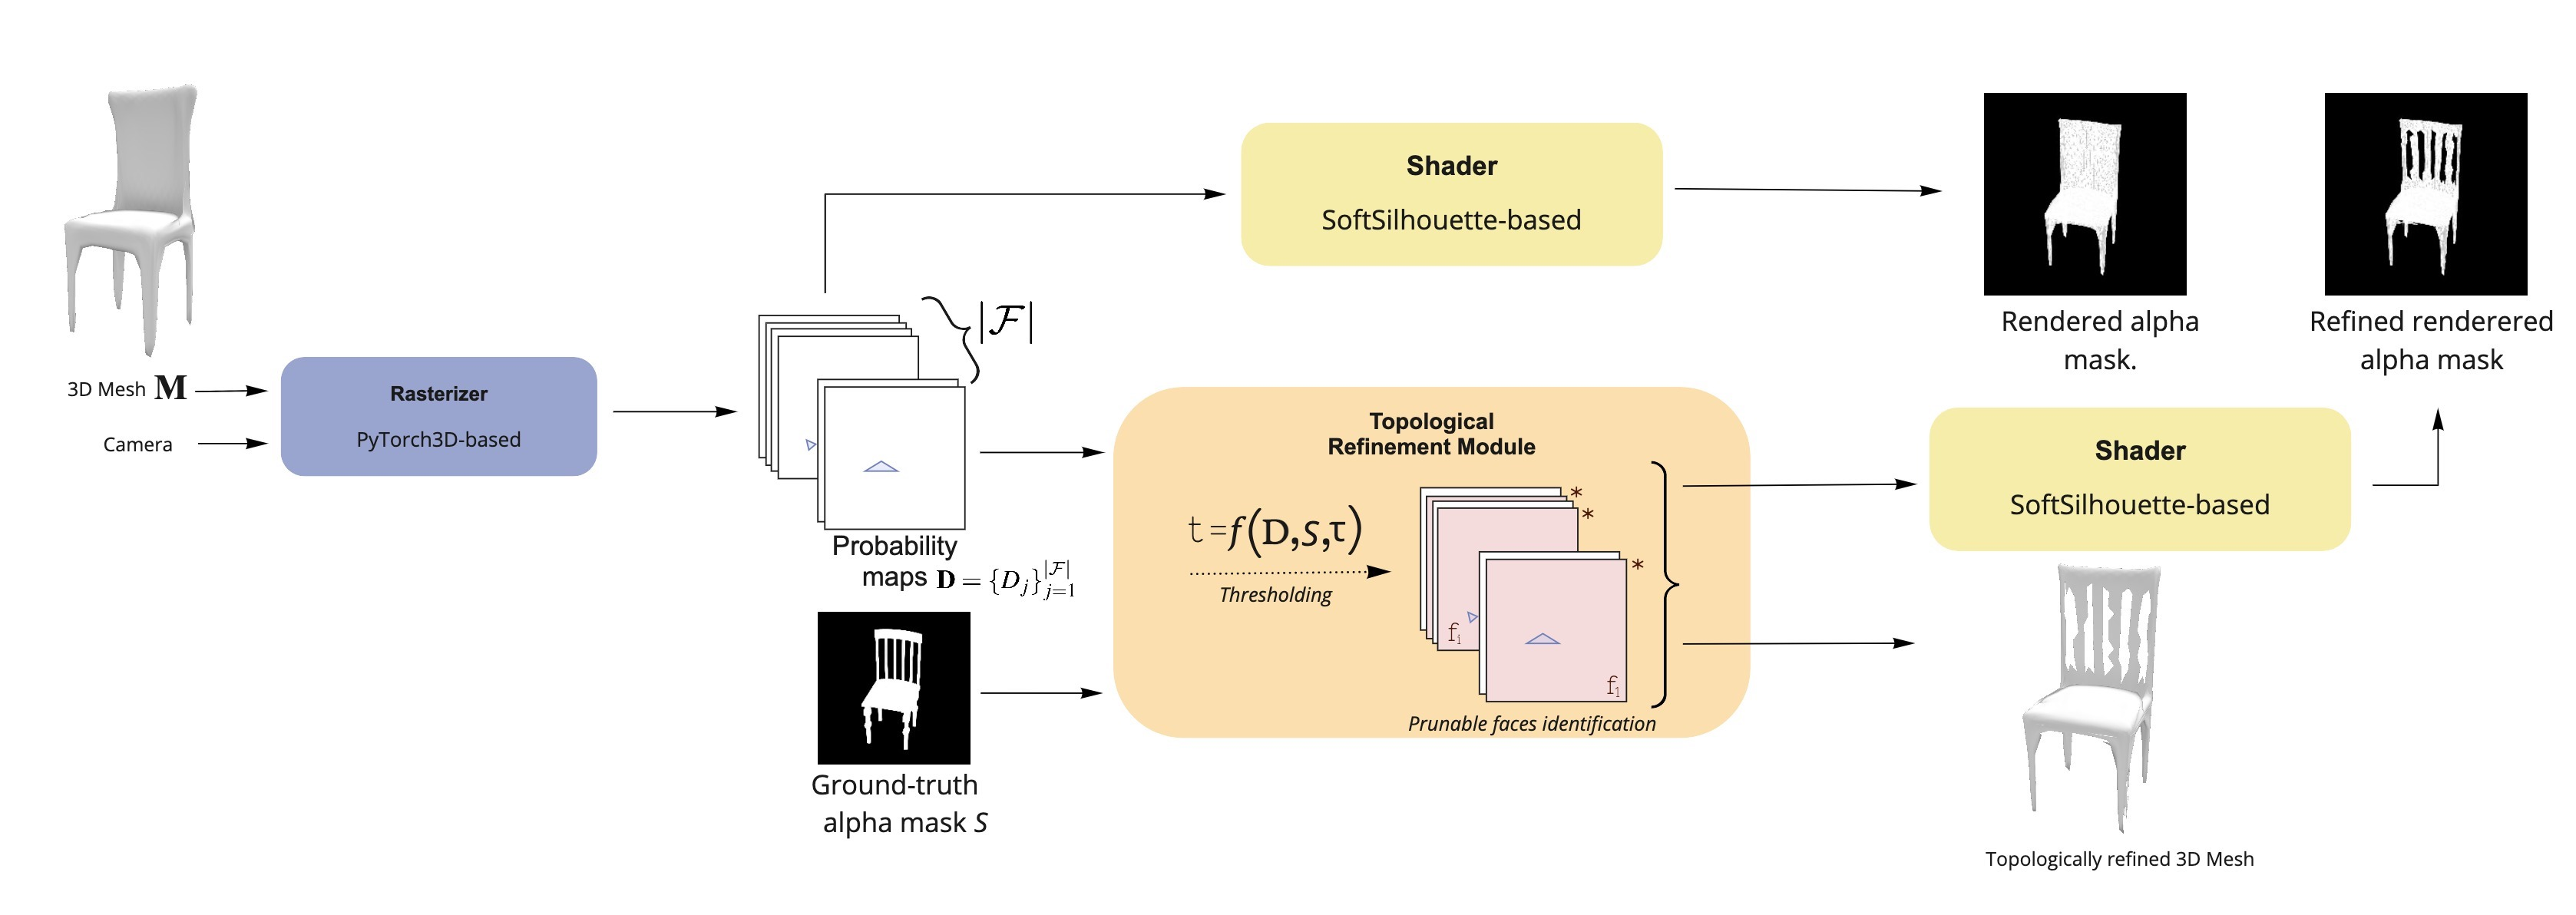
\includegraphics[width=\linewidth]{images/adaptativesr/final_figure.jpg}
\end{center}
    \caption{Architecture overview of our method. \textit{Based on a 3D mesh} \textbf{M} \textit{and a camera pose information, our module leverages onto PyTorch3D rasterizer to detect and prune onto the mesh surface by only getting consideration for the ground-truth alpha mask S}}
\label{fig:pipeline_overview}
\end{figure*}

Detecting those faces can be made through the computation of an Intersection over Union (IoU) score between the face from F involved in the rendering of \textbf{M} and the ground-truth alpha mask \textit{S}. Those faces can then be removed from the 3D mesh surface or directly discarded in the shader stage of the renderer. Inspired by the thresholding strategy introduced in \citep{pan2019deep}, we set an adaptative threshold $\tau$ based on the IoU score distribution and quantile $Q_{\tau}$ where $\tau \in [0,1]$.

\begin{equation}
    \tau=Q_{\tau}({\gamma/\Gamma})
\end{equation}

where ${\gamma/\Gamma}$ refers to the IoU distribution score. 
In a similar fashion line to what \citep{pan2019deep} did for the thresholding strategy in their pipeline architecture, the setting of $\tau$ influences the number of pruned faces: the lower $\tau$ is, the lower the number of faces detected as wrongly projected will be.

\paragraph{Implementation details.}
We implement our topological refinement strategy onto the renderer from the PyTorch3D \citep{ravi2020accelarating} library. The renderer's modularity offered by \citep{ravi2020accelarating} is worth mentioning since the entire rendering procedure can be adjusted as desired. We paid attention to its rasterization stage in our work for its connivance with the one from SoftRasterizer \citep{liu2019soft}. 

One of the core differences it exists between those two frameworks in the silhouette rasterization process concerns the number of faces involved: while PyTorch3D only considers for each pixel location $p_i$ the top-\textit{K} closest faces from the camera center of \textbf{M}, SoftRasterizer equally considers all the faces. 
We denote by $\mathbf{P}\in \mathbb{R}^{K\times(H\times W)}$ the intermediate probability map produced by \citep{ravi2020accelarating} which is highly related to the one originally introduced in \citep{liu2019soft}. Considering any 2D pixel location $p_{i}=(x_{i};y_{i}) \in \{0,..H-1\}\times\in \{0,..W-1\} $ and the $k^{th}$ closest face $f_{k}^{i}$, the distance based probability tensor $\mathbf{P}$ is expressed through:

\begin{equation}
    \mathbf{P}[k,p_{i}]=\left(1+e^{-d(f_{k}^{i},p_{i})/\sigma}\right)^{-1} 
\end{equation}

where $d(f_{k}^{i},p_{i})$ stands for the Euclidean distance between $p_i$ and $f_{k}^{i}$, while $\sigma$ is a hyperparameter to control the sharpness of the rendered silhouette image. Both $d$ and $\sigma$ have been defined in SoftRasterizer \citep{liu2019soft}. \newline

We consider the same soft silhouette shader stage as the one introduced in SoftRasterizer to obtain the soft alpha mask $\hat{S}$ from $\mathbf{P}$ through the aggregation function:

\begin{equation}
    \hat{S}[p_i]=1 - \prod_{k=1}^{K} (1 - \mathbf{P}[k,p_{i}])
\end{equation}

It is worth to emphasise the indexing notation in $\mathbf{P}$. Indeed, face indexes $f_{k}^{i}$ and $f_{k'}^{i'}$, $\{i,k\} \neq \{i',k'\}$ might refer to the same physical face on \textbf{M} because a rendered face is likely to cover an area larger than a single pixel. 

We introduced $\mathcal{F}$ as the set of unique faces involved in the rendering of any mesh \textbf{M} obtained from $\mathbf{P}$. The larger K is, the more likely the cardinality of $\mathcal{F}$ will get close to the total number of faces in the original mesh $|F|$. 

Finally and because $\mathbf{P}$ is not exactly designed in the same way as SoftRasterizer did, we denote by $\mathbf{D}=\{D_{j}\}_{j=1}^{|\mathcal{F}|}\in \mathbb{R}^{|\mathcal{F}|\times(H\times W)}$ the same probability map tensor as defined in \citep{liu2019soft}.

The way our module determined whether or not a face should be pruned is conditioned by the degree of overlap between the ground truth alpha mask \textit{S} and the rendered face. Since each face $f_{j} \in \mathcal{F}$ contributes to the final rendered silhouette through its probability map $D_{j}\in \mathbb{R}^{(H\times W)}$, an Intersection over Union (IoU) term is computed: 

\begin{equation}
\begin{cases}
     \gamma_{j}=\sum_{p_{i}\in S} \min \left(  D_{j}[p_{i}] , S[p_{i}] \right) \\
     \Gamma_{j}=\sum_{p_{i}\in S} \max \left( D_{j}[p_{i}],S[p_{i}] \right)
\end{cases}
\end{equation}

The ratio $\gamma_{j}/\Gamma_{j}$ gives the well-known IoU score. We extend the computation for a single face $f_{j}$ to all the faces from $\mathcal{F}$, and we note $\gamma/\Gamma \in \mathbb{R}^{|\mathcal{F}|}$ the complete IoU score distribution.

Our method finally leverages onto this distribution score to determine the faces which should be pruned on $\mathbf{M}$. We adopt a thresholding strategy partially inspired from \citep{pan2019deep} and set an adaptative threshold $t$ based on statistical quantile consideration: faces with a lower IoU score than $t=Q_{\tau}(\gamma/\Gamma)$ are pruned from $\mathbf{M}$. Such a choice allows to dynamically adapt the number of faces to prune based on the IoU distribution. 

\section{Experiments}
\label{sec:experiments}

\textbf{Dataset} Our approach has been extensively tested with the ShapeNetCore \citep{chang2015shapenet}. In line with the work from by TMN \citep{pan2019deep}, our experiments are thus restricted to the topologically challenging "chair" class from \citep{chang2015shapenet}. It contains a total of 6774 different chairs, with 1356 instances in the testing set.

\noindent\textbf{Metrics} We evaluate our method through both qualitative and quantitative considerations. We use the 2D IoU metric to assess how well the refined mesh produced by our module better match the ground truth alpha mask compared to the topologically non-refined mesh. We also use 3D metrics with the Chamfer Distance (CD), F-Score and METRO distance to evaluate our method. The METRO criterion is first introduced in \citep{cignoni1998metro} and reconsidered in Thibault Groueix \etal 's AtlasNet \citep{groueix2018papier} work. Its use is motivated by its consideration for mesh connectivity contrary to the CD or F-score metric that only reason onto 3D point clouds distribution. 

\noindent\textbf{3D Mesh generation network} Our refinement module can be integrated into any image-based 3D reconstruction pipeline and is thus agnostic to the network responsible for producing the 3D mesh. We chose to work with the meshes generated by \citep{pan2019deep} and thus trained it with the training set from \citep{chang2015shapenet}. Since we only want to focus on face-pruning considerations, we only train the ResNet18 encoder with the first stage of their 3D mesh reconstruction architecture, referred to as \textit{SubNet-1} in \citep{pan2019deep} and abbreviated as TMN in this section. The TMN architecture thus consists of a deformation network and a learnt topological modification module. It is worth mentioning the TMN \citep{pan2019deep} architecture has been trained and used for inference with the provided ground truth labels and rendered images from 3D-R2N2 \citep{choy20163d}. We called "Baseline" the deformation network preceding the topology modification network \citep{pan2019deep}. The genus-0 3D mesh produced by the Baseline network has been obtained from a 3D sphere template with 2562 vertices. 

\noindent\textbf{PyTorch3D Renderer} We use the PyTorch3D \citep{nie2020total3dunderstanding} differentiable renderer and set K=30 and $\sigma=5.10^{-7}$ to get the alpha mask as sharp as possible. All the 2D alpha masks, size 224x224, involved in this Experiments section were obtained with the PyTorch3D renderer and have been centred. Similarly to what \citep{choy20163d,liu2019soft,yan2016perspective} did for the rendering silhouette masks, we considered 24 views per meshes with a fixed camera distance $d_{camera}=2.732m$ and an elevation angle set to $30\degree$. The azimuth angle varies by an increment of $15\degree$ from $0\degree$ to $345\degree$. All the meshes predicted by pan2019deep \citep{pan2019deep} were normalised in the same way as ShapeNetCore\citep{chang2015shapenet}. 

We both present qualitative and quantitative results of our pruning based method through 2D and 3D evaluation considerations. We demonstrate how effective our method can be by only leveraging on 2D alpha masks and the renderer modularity. 

\paragraph{Topological refinement evaluation - Qualitative results.} We aim first to highlight to which extent we can detect the relevant faces on the 3D mesh that might be pruned during the rendering. Figure \ref{fig:face2prune} highlights the faces considered as wrongly rendered compared to the ground-truth alpha mask on three different chairs. Based on these 2D silhouette considerations, we achieve visually more appealing results than \citep{pan2019deep}. 

\begin{figure*}[htp!]%[htp!]
\begin{center}
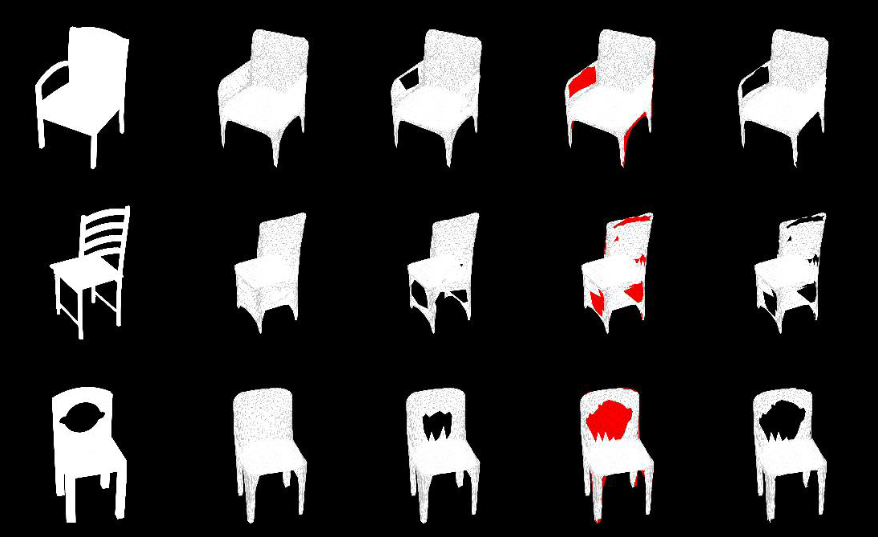
\includegraphics[width=\linewidth]{images/adaptativesr/highlight_faces.png}
\end{center}
    \caption{Silhouette based comparison on several instance from the ShapeNetCore test set. \textit{Faces rendered onto red regions should be pruned on 3D mesh surface} - $\tau = $ \textbf{0.05} - From left to right: Ground-Truth, Baseline, TMN\citep{pan2019deep}, Ours with highlighted faces to prune, Ours final result.}
\label{fig:face2prune}
\end{figure*}

The Figure \ref{fig:pruning_multi_view} somehow extends the later observation through 6 different viewpoints from the same chair instance. In this specific example, the TMN pruning module failed to detect some faces to prune. It produced the same mesh as the baseline one, while our method successfully pruned the faces that were rendered the worst, according to the ground truth alpha mask. The faces that are pruned on each view are independent of the other viewpoints. 

\begin{figure*}[htp!]%[htp!]
\begin{center}
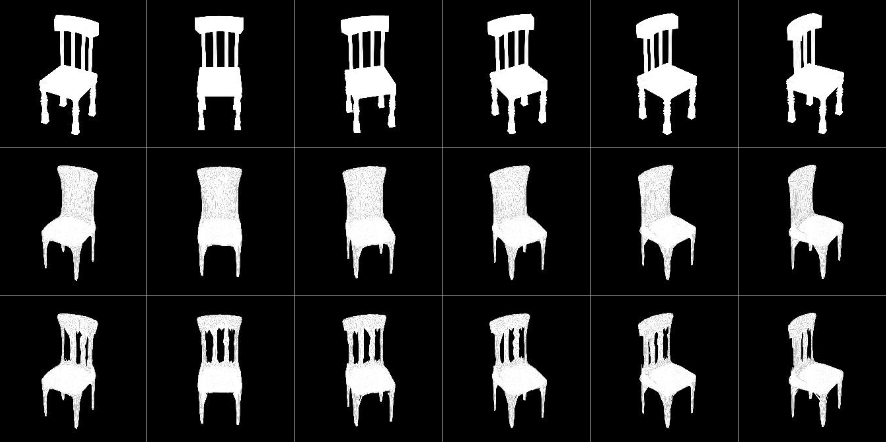
\includegraphics[width=\linewidth]{images/adaptativesr/severalview2D.png}
\end{center}
    \caption{Rendered silhouette mask results on 6 viewpoints - $\tau =\textbf{0.05}$ - From top to bottom: Ground-Truth, TMN\citep{pan2019deep},  Ours}
\label{fig:pruning_multi_view}
\end{figure*}

Even the viewpoint associated to a tricky azimuth angle as the one depicted in the last column is informative enough for our module to remove the relevant faces during rendering.

\paragraph{2D and 3D-based quantitative evaluation.} We compare the performances of our method through different threshold $\tau$ on Table \ref{tab:sota_table} with both the meshes produced by the Baseline network and TMN\citep{pan2019deep}. From the 1356 inferred meshes in the ShapeNetCore\citep{chang2015shapenet} test set, we manually selected 50 highly challenging meshes (from a topological perspective) and render them through the 24 different camera viewpoints we described earlier with the PyTorch3D's renderer. The threshold associated to the F-score has been set to 0.001. A total number of N=10.000 points have been uniformly sampled over the different meshes surface to compute the 3D metrics. 

\begin{table}[htp!]
    \caption{2D and 3D-based metric scores comparison with the Baseline and TMN \citep{pan2019deep} - \textit{Presented results were averaged over the 50 instance from our manually curated test set and over the 24 different viewpoints for the 3D metrics.} Best results are highlighted in \colorbox{red!25}{red}, second best in \colorbox{orange!25}{orange} and third ones in \colorbox{yellow!25}{yellow}.}
    \label{tab:sota_table}
    \begin{center}
    \centering
    \begin{adjustbox}{width=\textwidth}
    \begin{tabular}[h]{c||cccc}
    \hline
    Method \textit{(2D/3D supervision)} &  2D IoU ($\uparrow$) & CD ($\downarrow$) & F-Score ($\uparrow$) & METRO ($\downarrow$) \\[.5pt]
    \hline
    \textit{baseline} (-)& 0.660  &  6.602  & 53.27  &  1.419  \\[1.5pt]
    TMN \citep{pan2019deep} (3D)  & 0.681  & \cellcolor{red!25}{6.328}   & \cellcolor{red!25}{54.23}  & \cellcolor{red!25}{1.293} \\
    \hline 
    Ours $\scriptstyle \tau=0.01$ (2D) & 0.747 &\cellcolor{yellow!25}{6.541}  &  \cellcolor{orange!25}{53.39} &  1.418      \\
    Ours $\scriptstyle \tau=0.03$ (2D) & 0.755 &6.539  & \cellcolor{orange!25}{53.39}  &    \cellcolor{yellow!25}{1.417}  \\
    Ours $\scriptstyle \tau=0.05$ (2D) & \cellcolor{yellow!25}{0.763} & \cellcolor{orange!25}{6.540}  &  \cellcolor{yellow!25}{53.34} &   \cellcolor{yellow!25}{1.417}     \\
    Ours $\scriptstyle \tau=0.1$ (2D)& \cellcolor{red!25}{0.778} & 6.551  & 53.27 &  \cellcolor{orange!25}{1.416}     \\
    Ours $\scriptstyle \tau=0.15$ (2D)& \cellcolor{orange!25}{0.771} & 6.548  & 53.26  &    \cellcolor{orange!25}{1.416}   \\
    \hline 
    \end{tabular}
    \end{adjustbox}
    \end{center}
    
    \end{table}

Our method outperforms the learned topology modification network from TMN\citep{pan2019deep} according to Table \ref{tab:sota_table} when compared using the 2D IoU score. It is worth re-mentioning that the presented results for TMN\citep{pan2019deep} only come from the very first learned topological modification network and thus do not consider the topological refinement from the \textit{SubNet-2} and \textit{SubNet-3} network. Whereas none of our configurations (with different $\tau$ values) succeed to reach better scores on 3D metrics than TMN\citep{pan2019deep}, we stress on two points: \begin{enumerate}
    \item Topologically refined mesh by our method always get better results than the ones produced by the Baseline. 
    \item Our face-pruning strategy only relies on a single 2D alpha mask and does not required any form of 3D-supervised compared to \citep{pan2019deep}. 
\end{enumerate}

Since the method we designed only relies on 2D considerations, the camera viewpoint we considered to perform the topological refinement must influence the different evaluation metrics. We show in Figure \ref{fig:pruning_viewpoint_influence} to which extent the camera pose affects both the 2D IoU and the CD scores.

\begin{figure}[h!]
  \centering
  \subfloat[a][2D IoU]{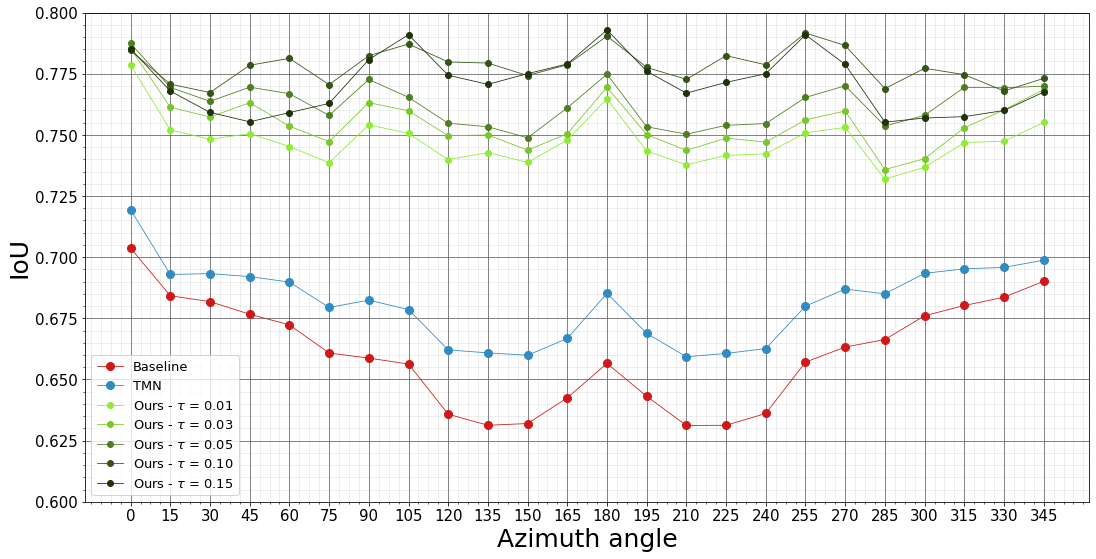
\includegraphics[width=\linewidth]{images/adaptativesr/multiviewsPLOT.png} \label{fig:a}} \\
  \subfloat[b][Chamfer distance]{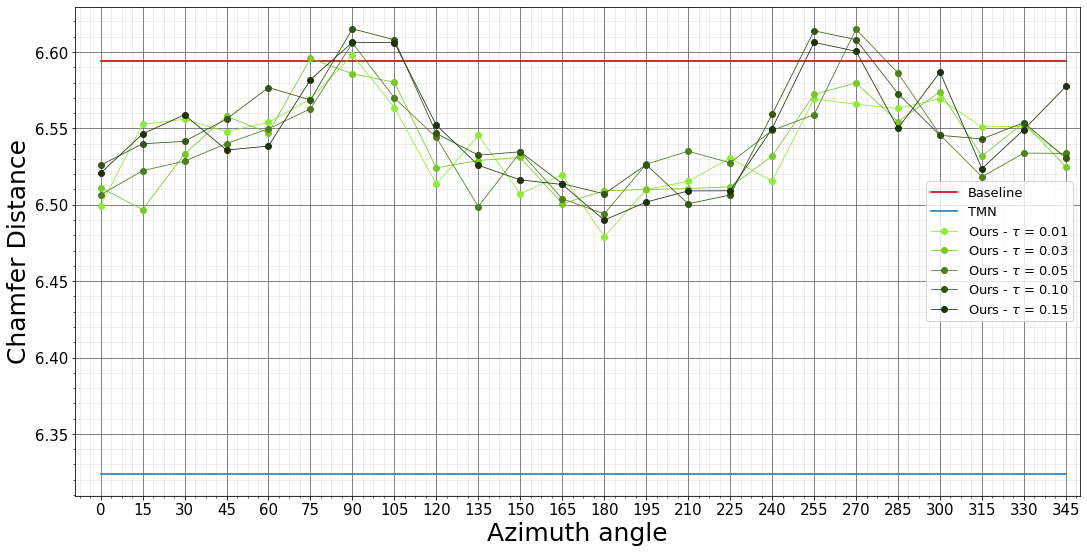
\includegraphics[width=\linewidth]{images/adaptativesr/plot_Chamfer_Distance_last.png} \label{fig:b}}
  \caption{Camera viewpoint influence over the 2D IoU (top, (a)) and Chamfer distance (bottom, (b)) scores.} \label{fig:pruning_viewpoint_influence}
\end{figure}

Azimuth angles around the symmetrical pair $\{90^{\degree}, 270^{\degree}\}$ are more challenging since there are not as informative as the viewpoints closed to $180^{\degree}$. Indeed, our method struggles to get better results than the Baseline on these cases. Our test set is slightly imbalanced since it only contains few chair instances where armrests require topological refinement and conversely a greater number with topologically complex back parts. Our method thus slightly performs worse than the Baseline on around both $90^{\degree}$ and $270^{\degree}$ angles as complex chairs' back structures are invisible on these viewpoints. 

We finally also quantitatively confirm the intuited impact of $\tau$ during the rendering process on the 2D IoU score: the higher $\tau$ is, the larger the number of faces we discarded. 


\subsection{Limitations and further work}

Our method shows encouraging results in 3D meshes topological refinement through 2D alpha mask considerations but has few remaining limitations. First regarding the thresholding strategy we used to determine whether or not a face should be pruned on the 3D mesh surface. While we require to set a fixed hyperparameter - $\tau$ - in our method as \citep{pan2019deep} did, we align with \citep{nie2020total3dunderstanding} on the importance to rely on local 2D and 3D prior information to propose a clever and more robust thresholding strategy. Moreover, our module might also incorrectly behave on the rendered faces closed to the silhouette boundary edges. 

From a broader work perspective, our method currently relies on alpha masks and thus leaves behind texture information from RGB images. While impressive 3D textured results exist with UV mapping on self-supervised image-based 3D reconstruction methods with genus-0 meshes\citep{li2020self,pavllo2020convolutional}, no attempts have been made to the best of our knowledge to go beyond such 0 order. Finally and since our work is completely agnostic to the 3D mesh reconstruction network, a natural next move would go for the design of a complete self-supervised 3D reconstruction pipeline where our topological refinement module is including. 

\subsection{Conclusion}
\label{sec:conclusion}
We proposed a new way to perform topological refinement onto 3D meshes surface by only getting consideration for 2D alpha mask and the modularity of the PyTorch3D rasterization framework. To the best of our knowledge, no attempt has been made in our line of work since both TMN\citep{pan2019deep} and Total3D\citep{nie2020total3dunderstanding} respectively perform faces and edges pruning through 3D-supervised  neural networks. In this way, our work introduced a new research path to address the 3D mesh topology refinement issue. The agnostic design of our method allows any self-supervised image-based 3D reconstruction pipeline - based on the PyTorch3D renderer framework - to leverage the work we presented in this paper to reconstruct topologically complex meshes. We obtained consistent and competitive results from a topological perspective compared to the 3D-based pruning strategy from \citep{pan2019deep}. 



\chapter{Additional ressource about EpipolarNVS}
\label{annex:epipolarnvs}

We provide in this annex some additional information regarding the Chapter ~\ref{chapter:epipolarnvs} and the EpipolarNVS model. 

\section{Dataset characteristics}
\label{annex:epipolarnvs-dataset}

Regarding the ShapeNet dataset, we decided to not use the same dataset as \citep{kim2020novel, sun2018multiview}  but rather worked with the rendered ShapeNet images from DISN \citep{xu2019disn}. It offers at least three main improvements over the ones used in \citep{kim2020novel}:

\begin{itemize}
    \item Intrinsic camera parameters are available. 
    \item Each object within a class has 36 different views (against 18 for the dataset provided by \cite{kim2020novel}). 
    \item Rendered images have a non null elevation angle and the azimuth one is sampled on a regular 10°  basis. A random noise term is added on each rendered view to slightly jitter the camera pose. 
\end{itemize}

Considering real-world Synthia \citep{ros2016synthia} and KITTI \citep{geiger2012we} datasets, original images used in \citep{kim2020novel} also only contain extrinsic matrices, leaving apart the intrinsic information our architecture requires. We, therefore, build up our own train/test sets, with the same scenes as the ones used in \citep{kim2020novel}. Images were resized to $256\times256$ for speed-up and convenience purposes and ground-truth intrinsic matrices were adjusted accordingly. Images we work with on these real scene scenarios are more challenging than the ones used in \citep{kim2020novel,sun2018multiview} since dealing with center-cropped images discards fast-moving elements (on image borders) from the scenes.

Finally, we get consideration for the same setting used in \citep{kim2020novel} for the maximal latitude between the source and target view: full $\pm 180^{\circ}$ azimuthal range is permitted for the ShapeNet classes while a maximum of $\pm 10$ frames are considered for the real world datasets Synthia \citep{ros2016synthia} and KITTI \citep{geiger2012we}.

\section{Inference results}
We finally present in this last part additional qualitative results from our model, on all the four datasets we have get consideration for in this study. We present for each dataset 8 different scenes or object instances. 

\begin{figure*}[htp!]
    \begin{center}
    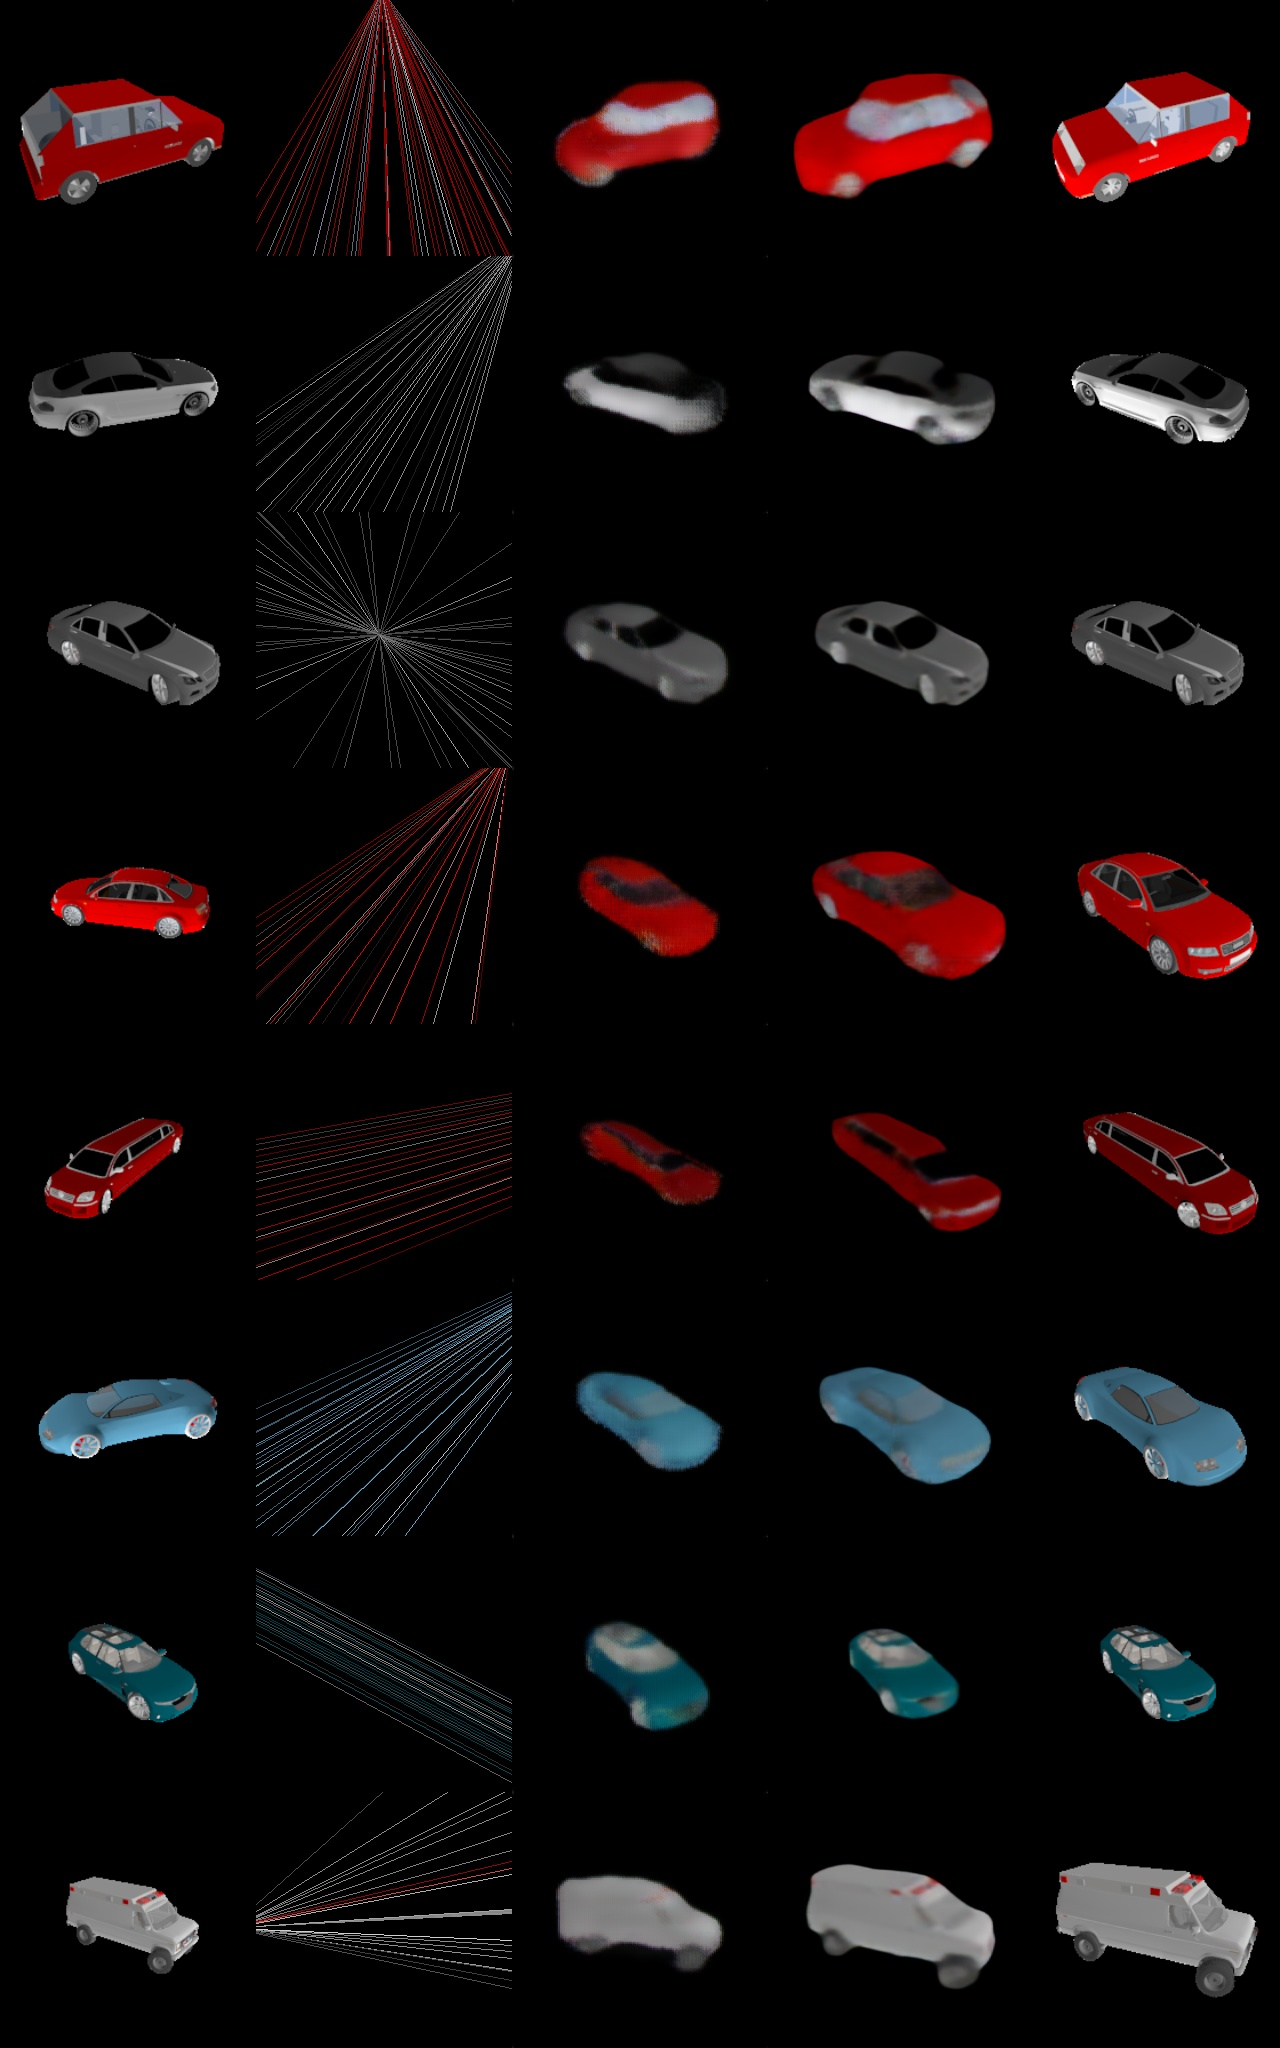
\includegraphics[width=.9\textwidth]{images/epipolarnvs/SuppMat_Car.jpg}
    \end{center}
     \caption{Visual results from the test ShapeNet ~\cite{Shapenet} \textit{Car} class. From left to right: the source image  $I_s$, the Encoded Pose $E_{s\xrightarrow{}t}$,  the prediction of ~\cite{NVS_skip}, our prediction and the target image $I_t$.}     \label{fig:add_visCar}
\end{figure*}

\begin{figure*}[htp!]
    \begin{center}
    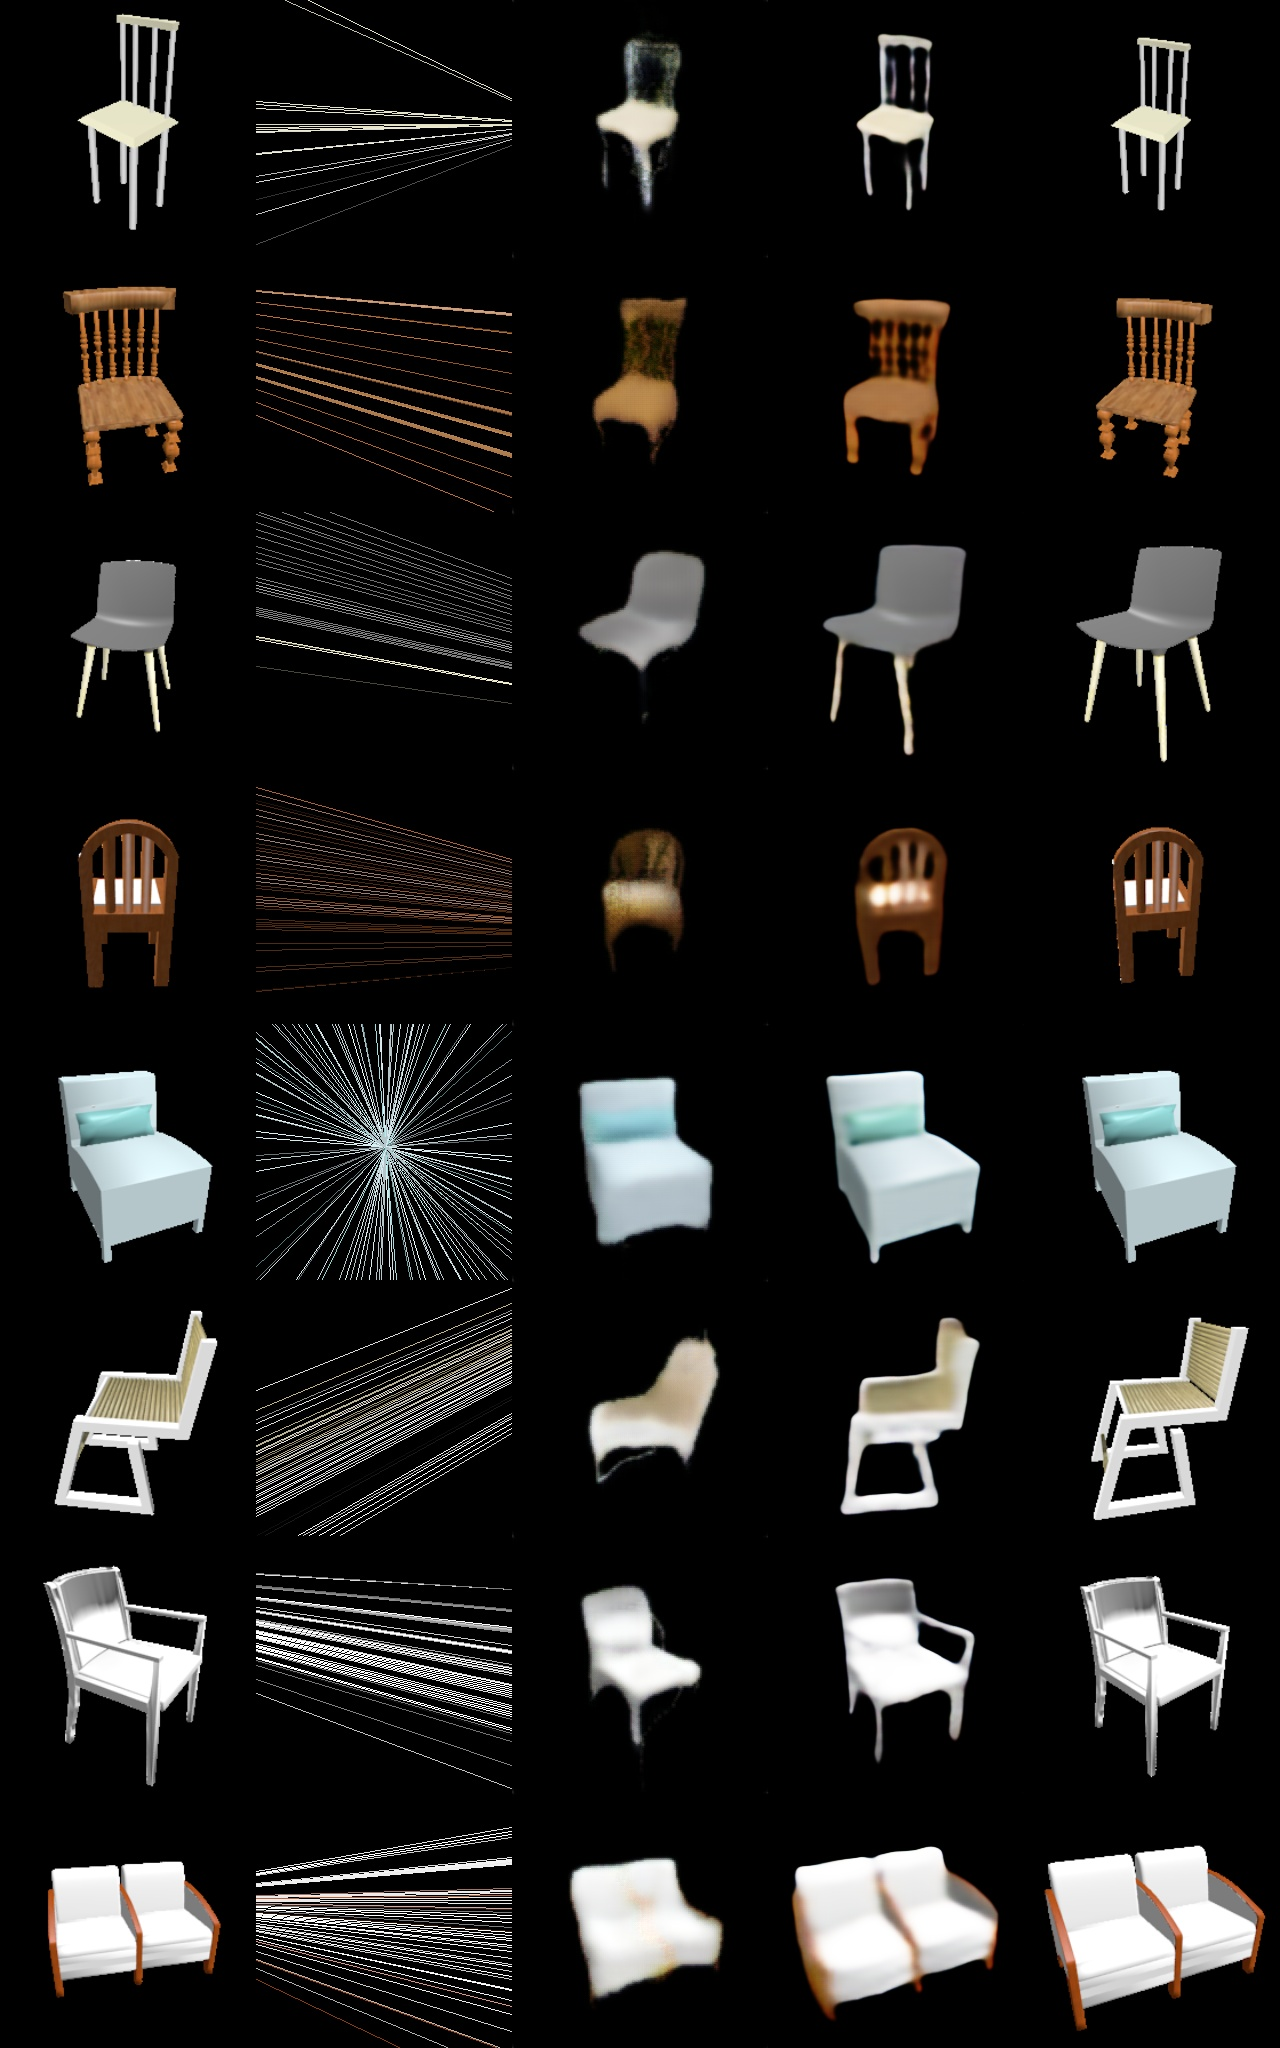
\includegraphics[width=.9\textwidth]{images/epipolarnvs/SuppMat_Chair.jpg}
    \end{center}
     \caption{Visual results from the test ShapeNet ~\cite{Shapenet} \textit{Chair} class. From left to right: the source image  $I_s$, the Encoded Pose $E_{s\xrightarrow{}t}$,  the prediction of ~\cite{NVS_skip}, our prediction and the target image $I_t$.}
     \label{fig:add_visChair}
\end{figure*}

\begin{figure*}[htp!]
    \begin{center}
    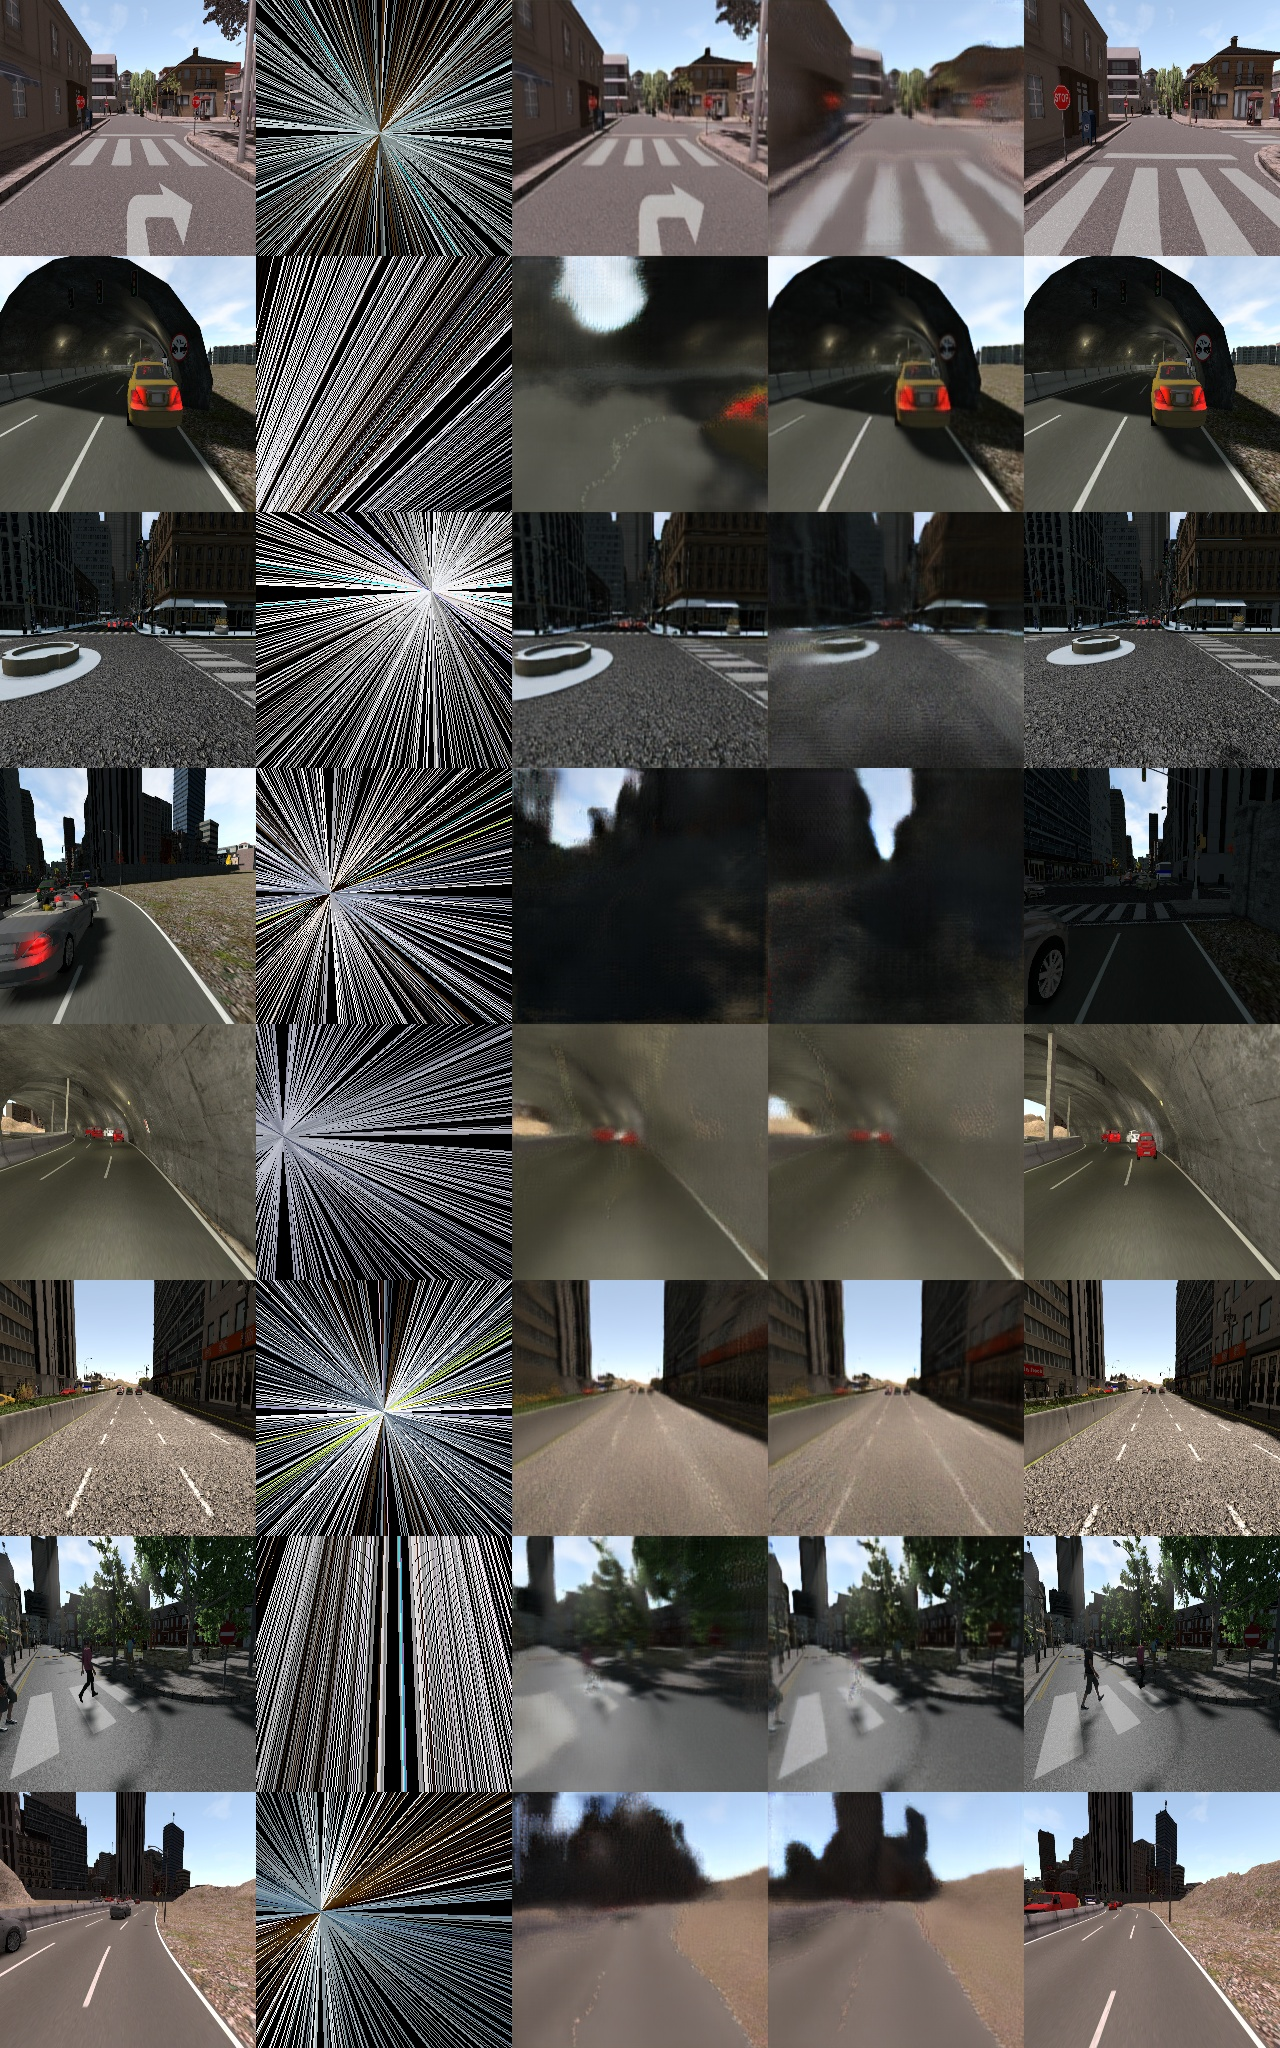
\includegraphics[width=.9\textwidth]{images/epipolarnvs/SuppMat_Synthia.jpg}
    \end{center}
     \caption{Visual results from the Synthia ~\cite{Synthia} test set. From left to right: the source image  $I_s$, the Encoded Pose $E_{s\xrightarrow{}t}$,  the prediction of ~\cite{NVS_skip}, our prediction and the target image $I_t$.}
     \label{fig:add_visSynthia}
\end{figure*}

\begin{figure*}[htp!]
    \begin{center}
    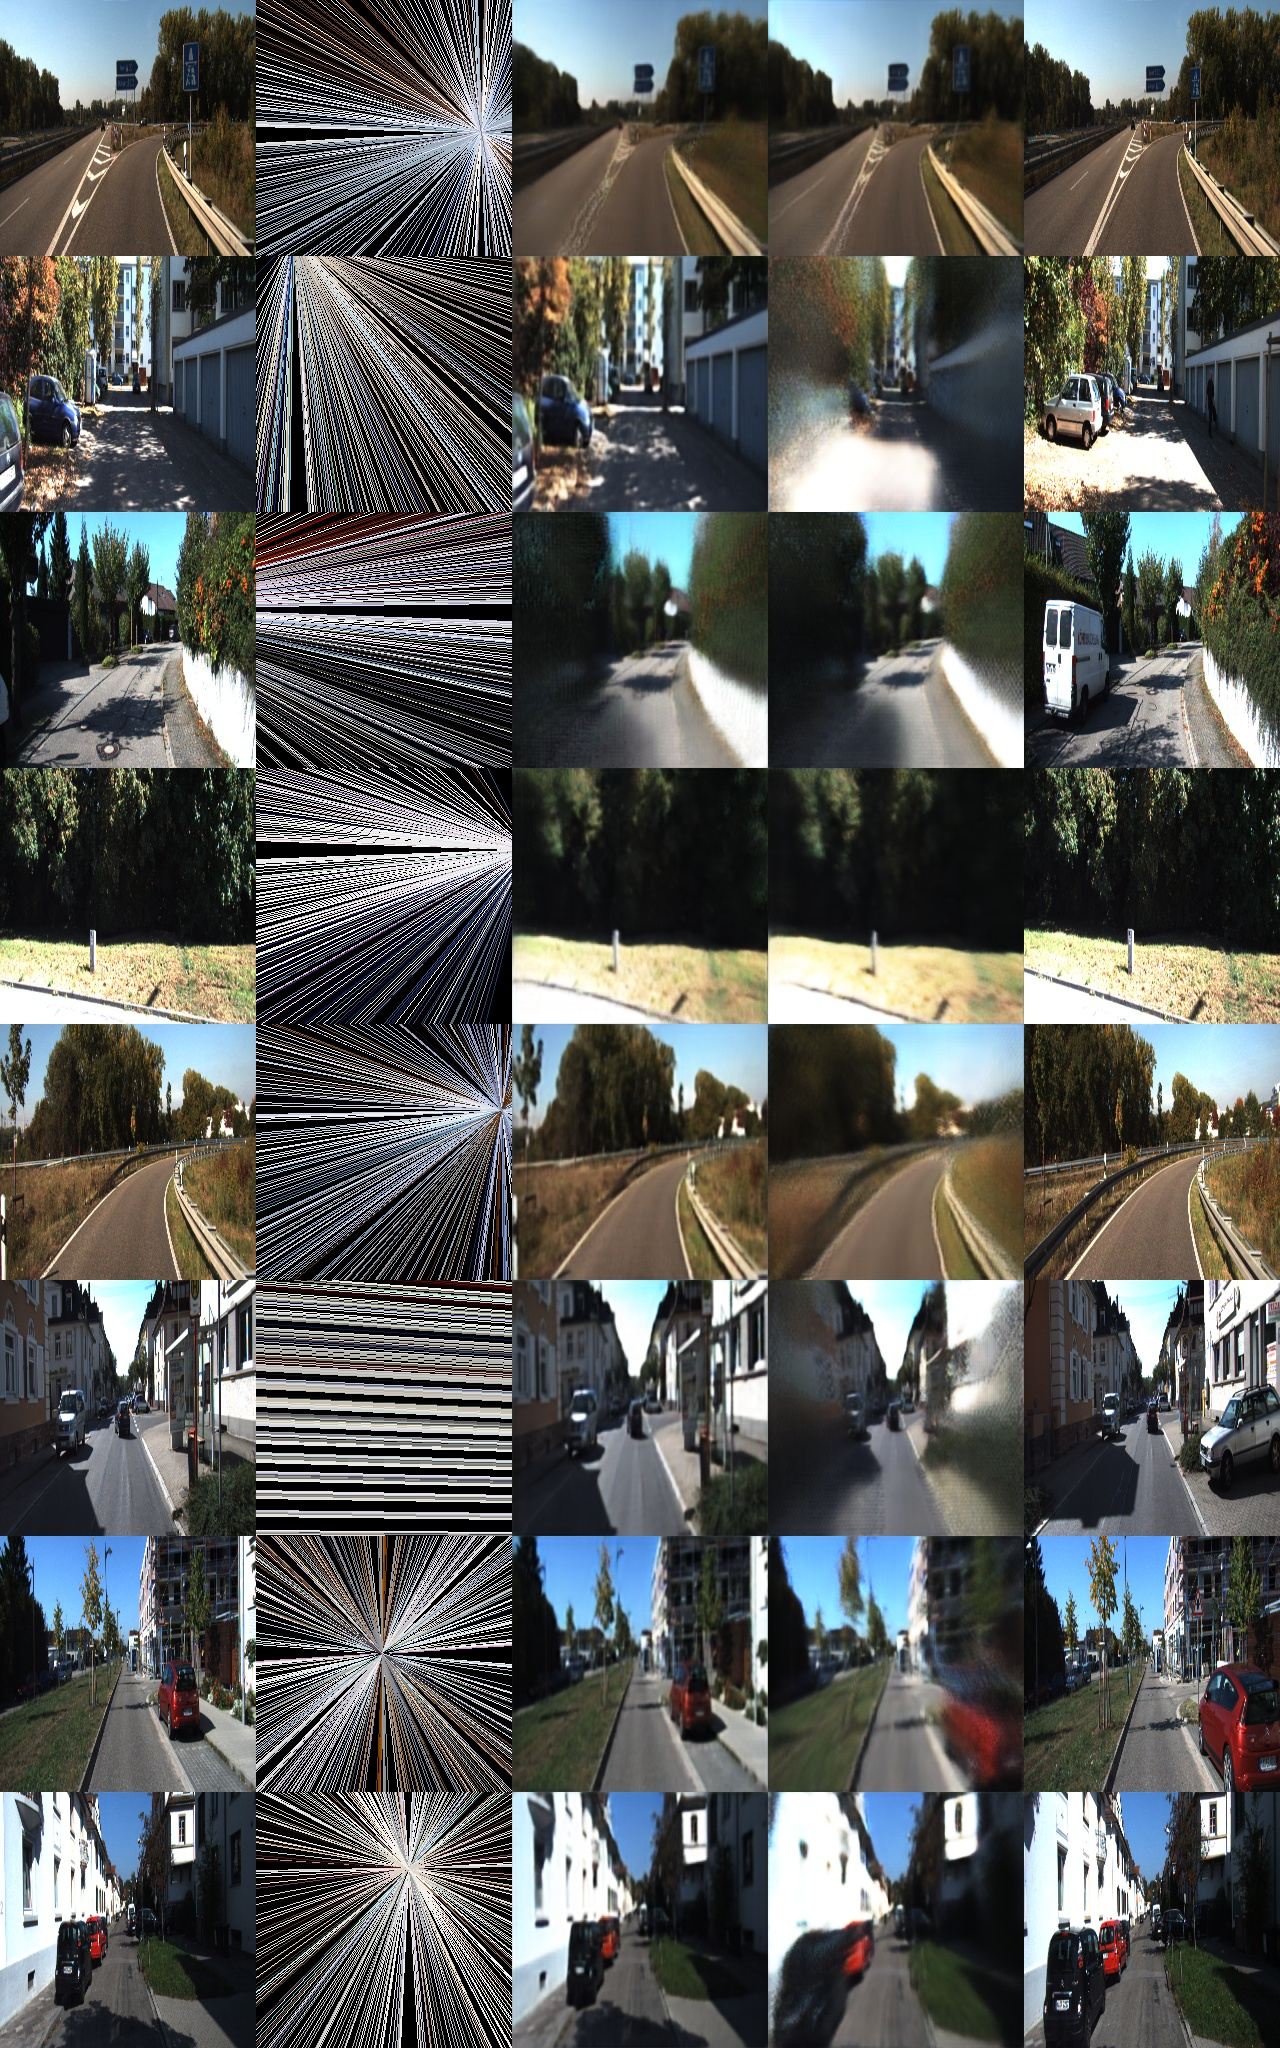
\includegraphics[width=.9\textwidth]{images/epipolarnvs/SuppMat_KITTI.jpg}
    \end{center}
     \caption{Visual results from the KITTI ~\cite{KITTI} test set. From left to right: the source image  $I_s$, the Encoded Pose $E_{s\xrightarrow{}t}$,  the prediction of ~\cite{NVS_skip}, our prediction and the target image $I_t$.}
     \label{fig:add_visKITTI}
\end{figure*}


\chapter{Additional ressource about EpiNeRF}

Further details about Chapter ~\ref{chapter:epinerf}, including EpiNeRF internal structure, training process, and view synthesis performance, are provided in this annex. 

\section{EpiNeRF submodules and training}

\subsection{Feature radiance fields: NeRFeature $\Psi$}

NeRFeature's internal architecture is illustrated in Figure \ref{fig:supp_nerfeature}. It closely mirrors the radiance structure of $\Phi$, even though there is no hypernetwork to predict its weights. NeRFeature is designed to produce deep features that lie in the latent space learned by $\chi$, similar to the approach implemented by \cite{ye2023featurenerf} through its distillation of foundation models \cite{oquab2023dinov2}. Our feature distillation strategy transfers information from the 2D model $\chi$ into 3D.  
\begin{figure}[htp!]
    \begin{center}
  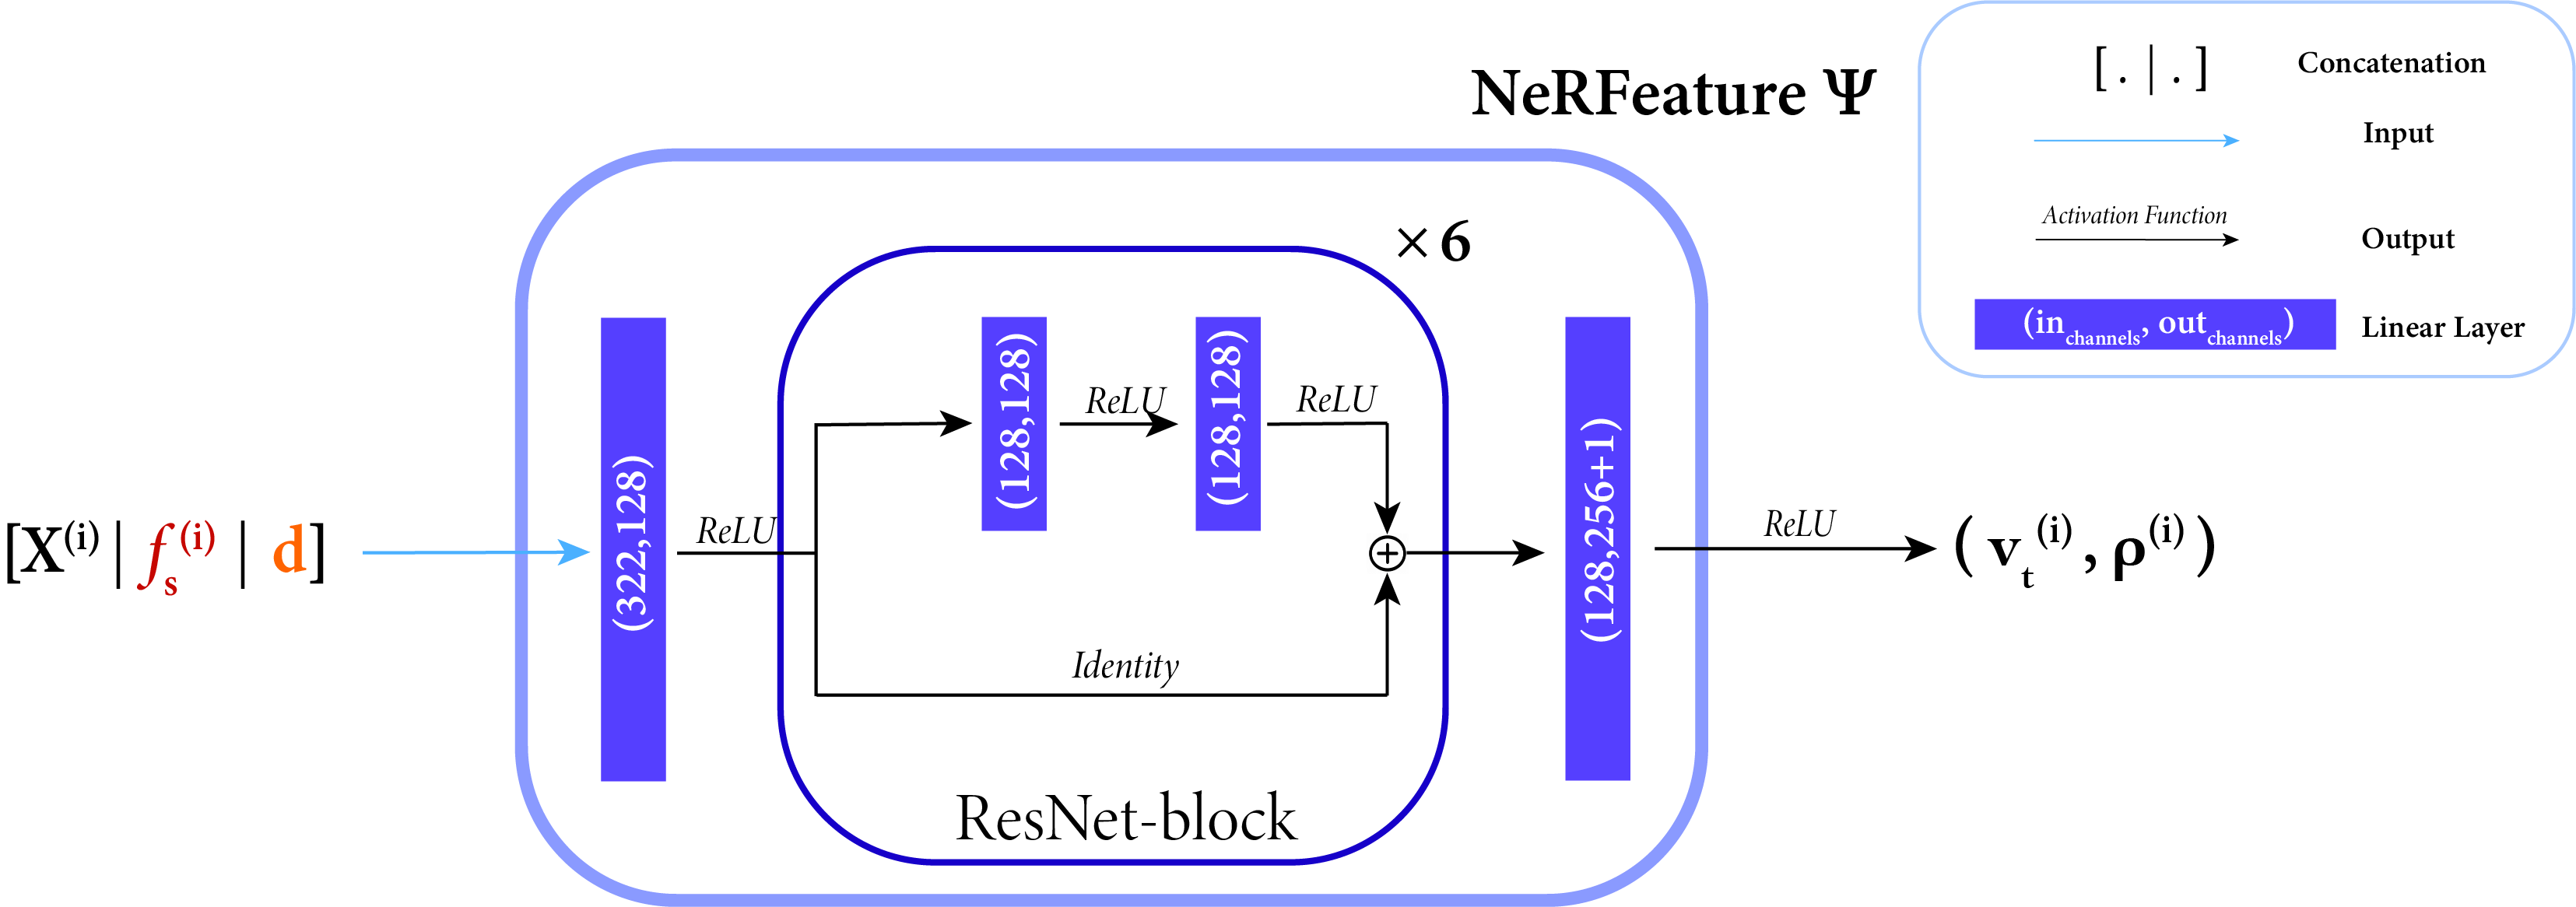
\includegraphics[width=\linewidth]{images/epinerf/supp_nerfeature.png}
  \caption{\textbf{NeRFeature overview.} NeRFeature implements a six ResNet blocks with an extended output that lives in $\mathbb{R}^{d_{\text{feat}}}$. Such an intermediate dense feature, with a transparency scalar, is later involved in the volume rendering operation to get $f_{t}$.}
  \label{fig:supp_nerfeature}
  \end{center}
\end{figure}


We get the final target-aligned deep feature from the vanilla volume rendering equation:

\begin{equation}
\label{eq:ft_vr}
    f_{t} = \sum_{i=1}^{N_{s}} T^{(i)}(1-exp(-\rho^{(i)}\delta_{i}))\mathbf{v}_{t}^{(i)} \in \mathbb{R}^{d_{\text{feat}}}
\end{equation}
with $T^{(i)} = \exp\left(-\sum_{j=1}^{i}\rho^{(j)}\delta_{j}\right)$ the accumulated transmittance along \textbf{r}.

As shown in Figure \ref{fig:supp_nerfeature}, the symmetrical pixel-wise feature $f_{s,symm}^{(i)}$ is not used as input for NeRFeature $\Psi$. Integrate a 3D symmetry prior into a high-dimensional space like $\mathbb{R}^{d_{\text{feat}}}$ is more complex than in the RGB space of $\Phi$. Instead, NeRFeature only receives a 3D point location, a direction, and the source-aligned feature $f_{s}^{(i)}$ as input.

\subsection{Epipolar-based feature attention}
This section gives additional explanations about our light feature attention mechanism.

As introduced in the main paper, the target-aligned features $\mathbf{f}{t}$ and the source-aligned one $\mathbf{f}{s}^{(i)}$ are used to compute the light cross-attention score $\mathbf{s}_{a}^{(i)}$:

\begin{equation}
    s_{a}^{(i)} = \frac{\mathbf{q}^{T}\mathbf{k}}{\sqrt{d_{\text{feat}}}}= \frac{f_{t}^{T}\times f_{s}^{(i)}}{\sqrt{d_{\text{feat}}}}
\label{eq:attention}
\end{equation}
while $\mathbf{s}_{a}$ denotes the entire distribution over all the points sampled along the ray \textbf{r}.

However, the cross-attention distribution $\mathbf{s}_{a}$ cannot be used directly in the volume rendering equation. The distribution lacks the sharpness needed to effectively influence the volume rendering process. It must be shrunk and normalized around its maxima in a differentiable manner to produce the final distribution $\hat{\mathbf{s}_{a}}$\footnote{Simplified as $\mathbf{s}_{a}$ in the main paper for convenience.}.

We thus designed two scaled sigmoid functions, called $S^{k}$ and $S^{K}$ to shrink $\mathbf{s}_{a}$ : 

\begin{align}
\hat{\textbf{s}}_{a} &= S^{K}(\textbf{s}_{a})\times S^{k}(\textbf{s}_{a}) \\
S^{q}(\mathbf{s}_{a}) &= \left(1- e^{q(\mathbf{s}_{a}-a_{0})}\right)^{-1}
\end{align}

where $q=\{k,K\}$ controls the sigmoid slope strength. \newline

The term $a_{0}$ adjusts the sigmoid midpoint value from 0.5 to $a_{0}$. Figure \ref{fig:attention_sigmoid} reflects these equations. Hyper-parameter $a_{0}$ allows to push attention scores that are lower than  $a_{0}$ toward 0.0 while attention that are higher than $a_{0}$ are thus drived against the maximum attention, set to 1.0 since the cross-attention distribution has been [0-1] normalized. We empirically set $k=10$, $K=60$ and $a_{0}=0.8$ during the EpiNeRF fine-tuning stage.\newline

\begin{figure}[h!]
    \begin{center}
  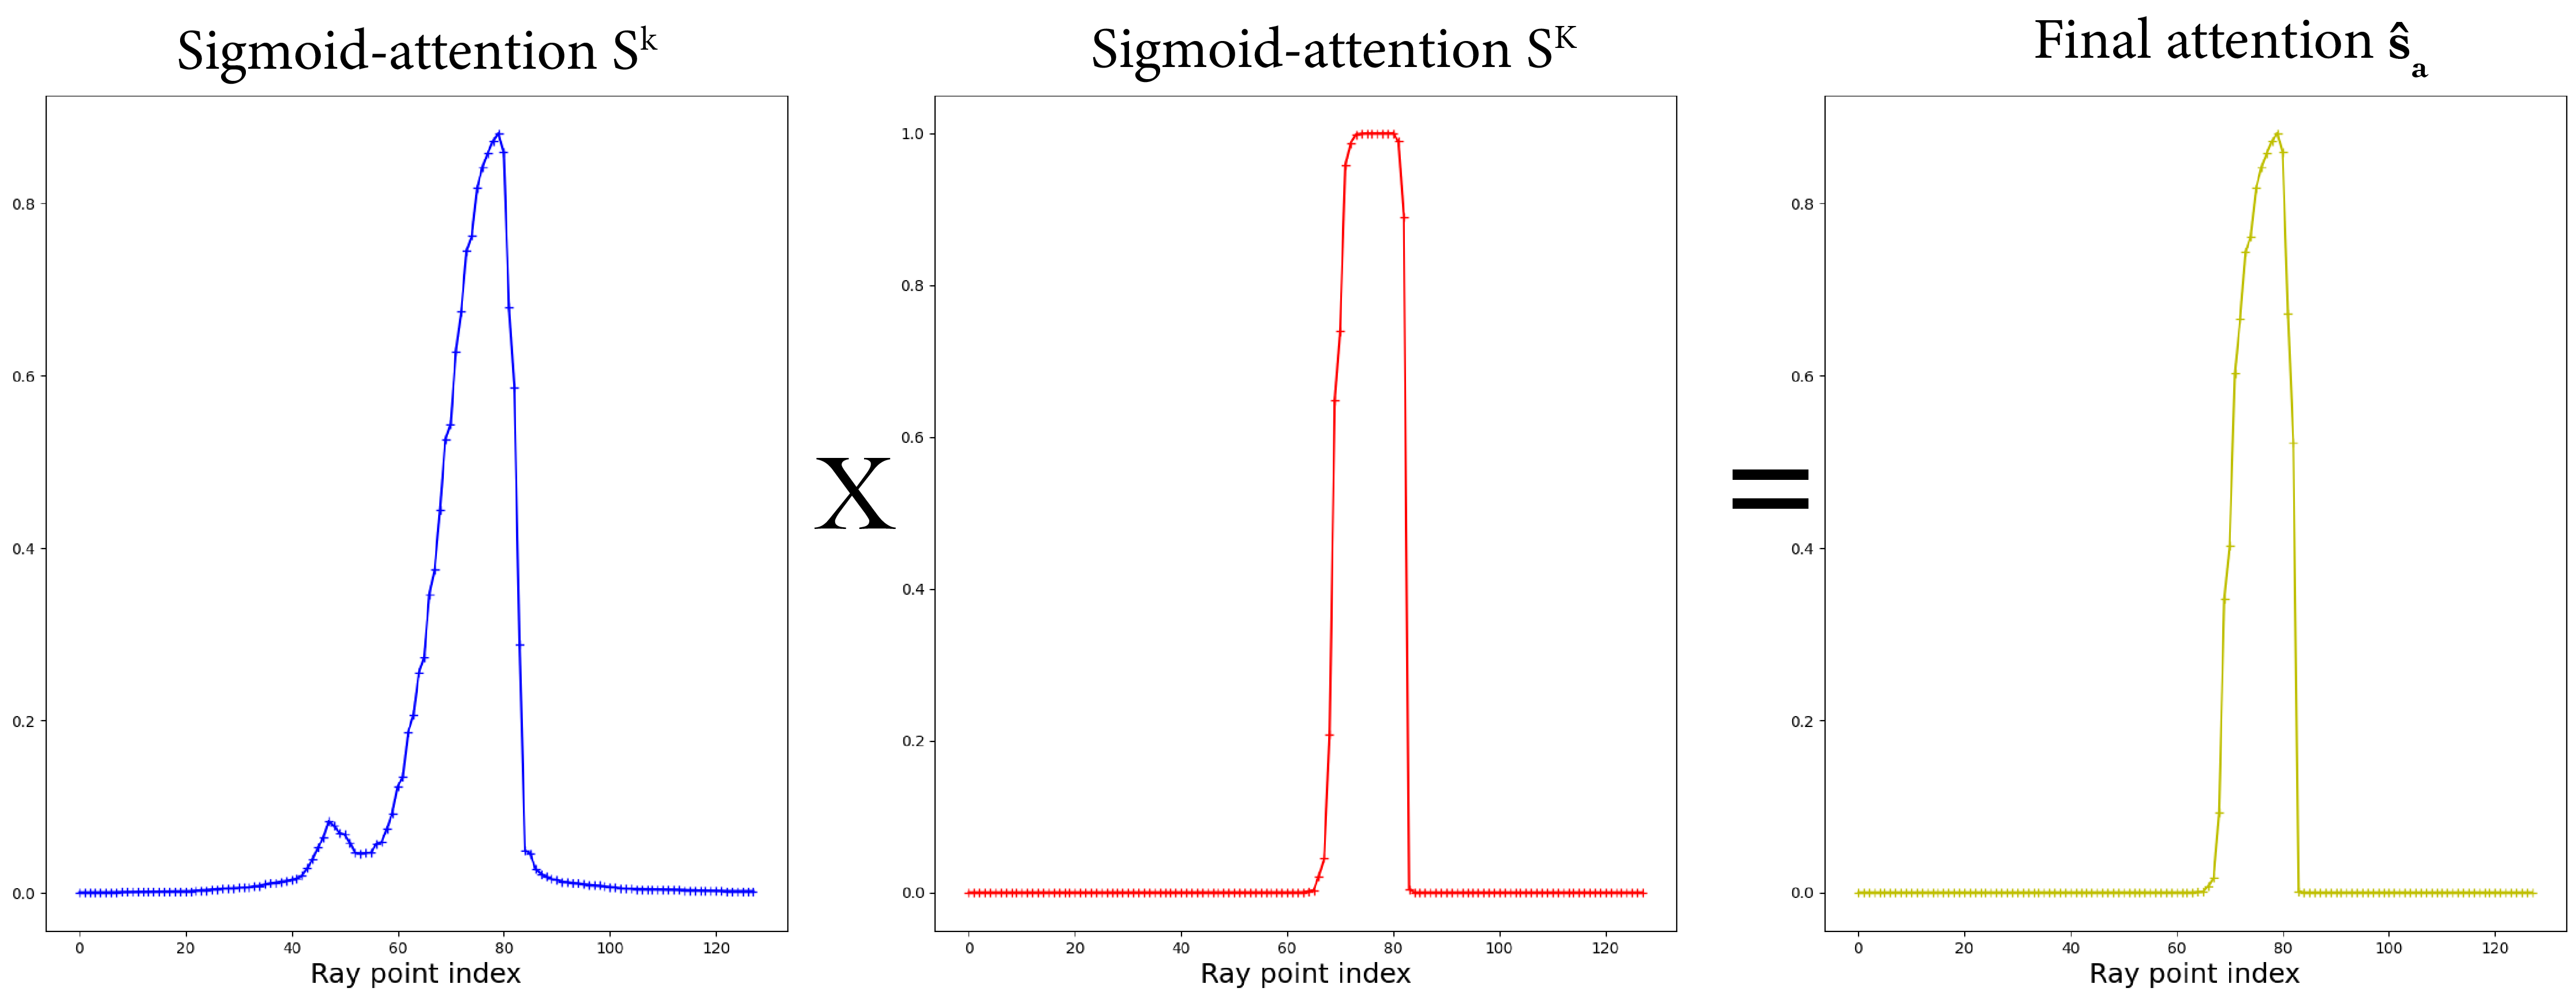
\includegraphics[width=\linewidth]{images/epinerf/SUPP_ATT_OVERLEAF.png}
  \caption{\textbf{Sigmoid shrinkage influence over} $\textbf{s}_{a}$. Intermediate attention distributions $S^{k}$ (\textit{left}) and $S^{K}$ (\textit{center}) allow to get $\hat{\mathbf{s}_{a}}$ (\textit{right}), the final attention distribution involved in the EpiNeRF architecture.}
  \label{fig:attention_sigmoid}
  \end{center}
\end{figure}

We finally illustrate on Figure \ref{fig:attention_construction} the $\alpha$-blending operation we perform in the main paper through the Equation \ref{eq:alpha}. 

\begin{figure}[h!]
    \begin{center}
  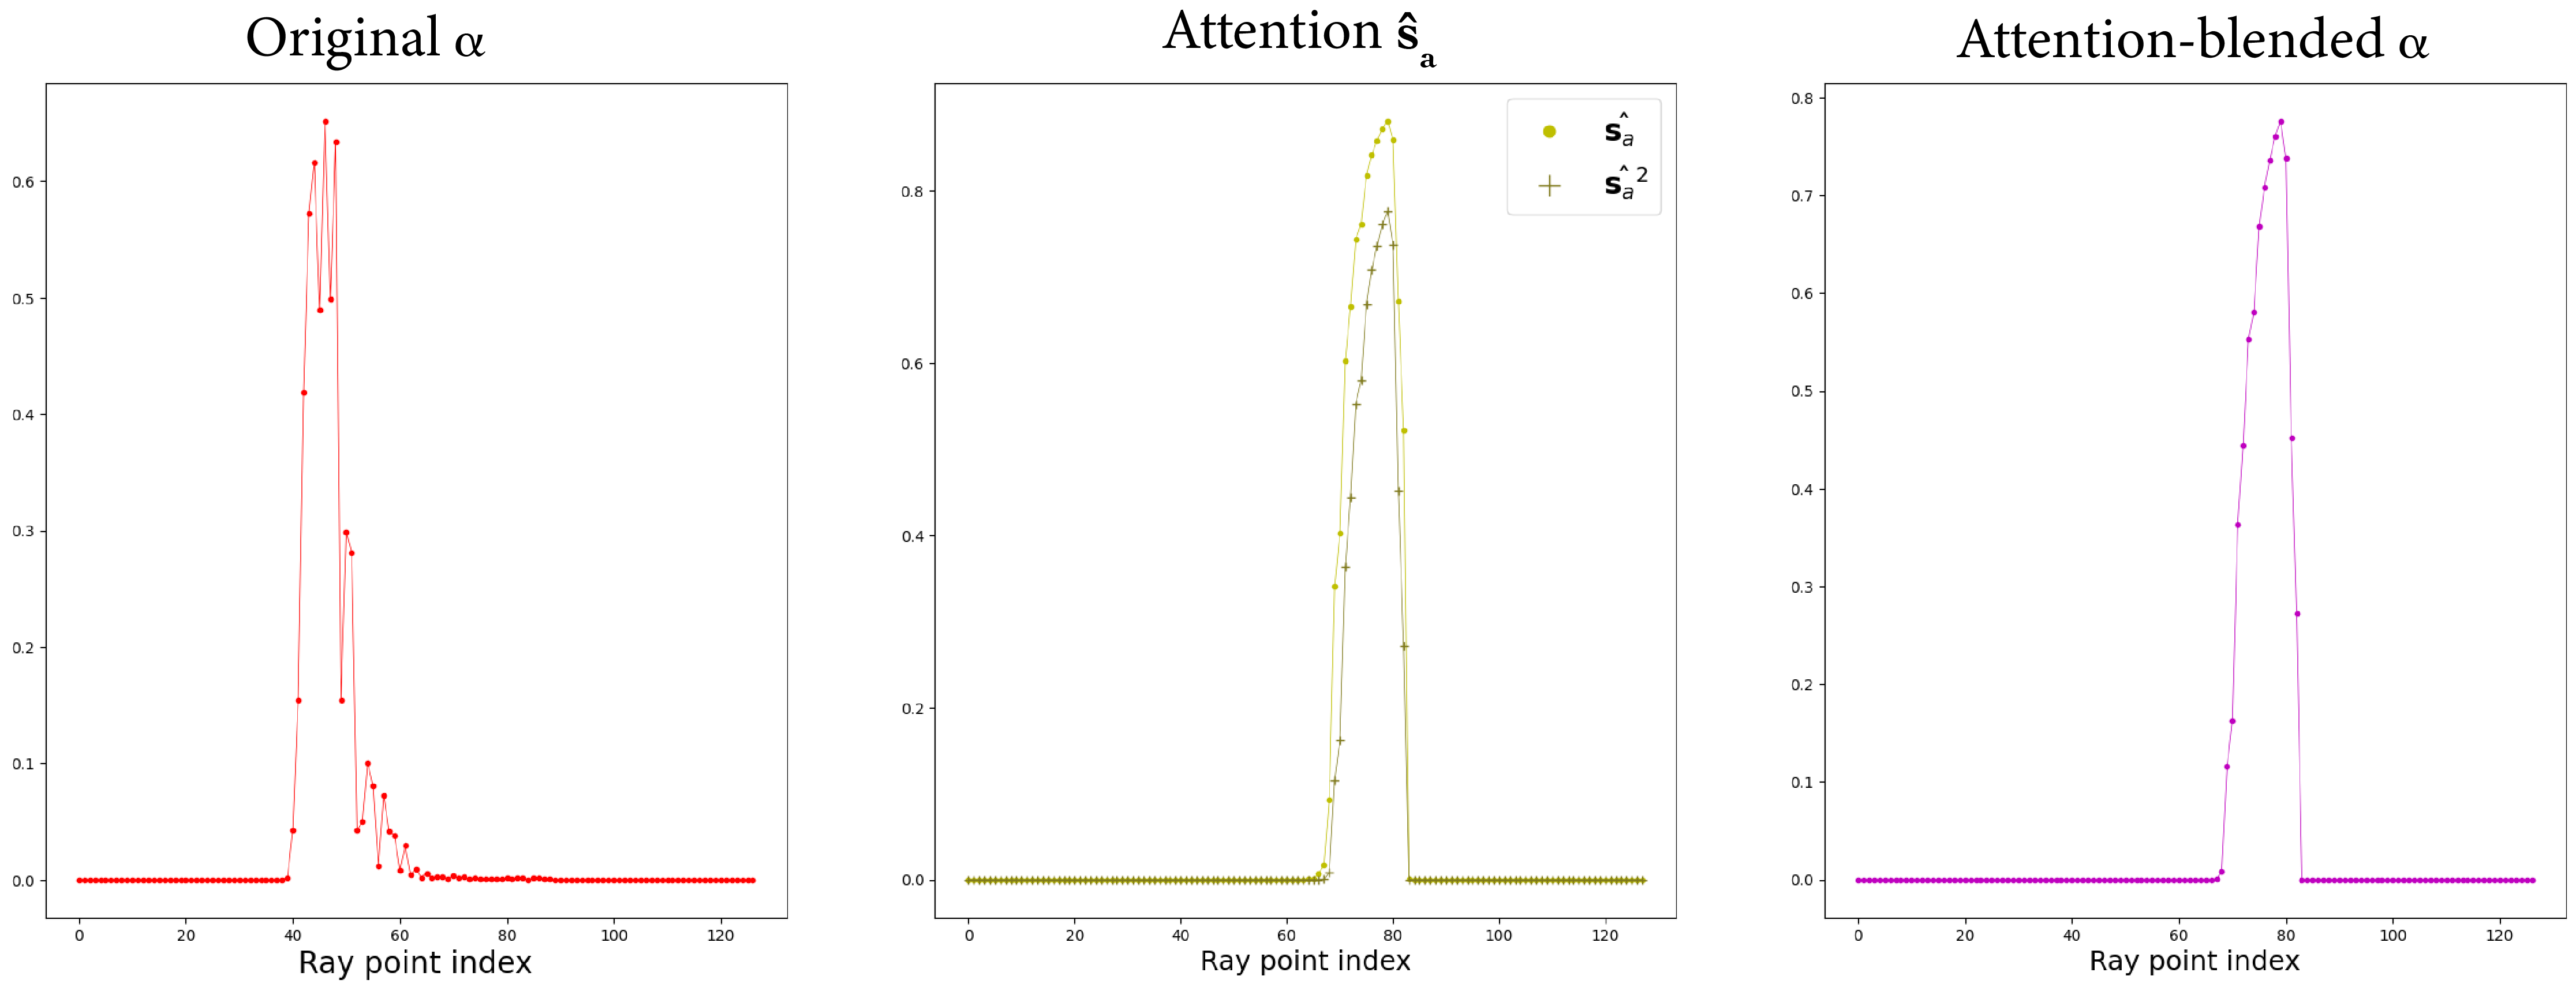
\includegraphics[width=\linewidth]{images/epinerf/SUPP_BLENDED_OVERLEAF.png}
  \caption{$\alpha$\textbf{-blending correction.} Original $\alpha$ distribution (\textit{left}) and its corrected attention-based counterpart (\textit{right}) show different activation regions along the ray. Cross-attention distributions $\hat{\textbf{s}}_{a}$ and $\hat{\textbf{s}}_{a}^{2}$ are plotted in the \textit{center} panel.}
  \label{fig:attention_construction}
  \end{center}
\end{figure}

The EpiNeRF epipolar cross-attention module aims to focus on regions where the attention $\hat{\textbf{s}}_{a}$ reaches its maximum values. As observed in Figure \ref{fig:attention_construction}, the blending operation shifts the $\alpha$ distribution slightly further away along the ray than it was originally. As expressed in Equation \ref{eq:weights} and illustrated in the main paper with the Figure \ref{fig:overall_attention}, the transmittance T is naturally affected by this shift correction. 

\subsection{Training details}
Although our EpiNeRF architecture requires several intermediate training steps, we expand the training losses already expressed in Equations \ref{eq:nerfeature_loss} and \ref{eq:epinerf_loss}. Regarding NeRFeature, the L2-loss is given by: 

\begin{equation}
\begin{split}
 \mathcal{L}_{\Psi}&= \sum_{\mathbf{r}\in\mathcal{R}} || f_{t}(\mathbf{r}) - \underbrace{f_{t}^{(GT)}(\mathbf{r})}_{=\mathbf{F}_{t}(\pi(\mathbf{r}))} ||_{2}^{2} 
\end{split}
\end{equation}

with $\mathbf{F}_{t} = \chi(I_{t})$. The final target-aligned deep feature $f_{t}$ is expressed in Equation \ref{eq:ft_vr}. \newline

Concerning EpiNeRF final training, we get the loss function: 

\begin{equation}
\begin{split}
 \mathcal{L}_{\zeta}= \sum_{\mathbf{r}\in\mathcal{R}} || c(\mathbf{r}) - \underbrace{c^{(GT)}(\mathbf{r})}_{= I_{t}(\pi(\mathbf{r}))} ||_{2}^{2}
\end{split}
\end{equation}
with $\zeta = \{\chi,\Phi,\Gamma\}$. Predicted colour $c(\mathbf{r})$ can be decomposed through the volumetric rendering equation as: 

\begin{equation}
c(\mathbf{r}) = \sum_{X^{(i)} \in \mathbf{r}}T^{(i)}\alpha^{(i)}c(\mathbf{X}^{(i)},\mathbf{d},\underbrace{f_{s}^{(i)},f_{s,symm}^{(i)}}_{= \mathbf{F}_{s}(\pi(X^{(i)})), \mathbf{F}_{s}(\pi(\mathbf{M}X^{(i)}))})
\end{equation}
and
\begin{equation}
\alpha^{(i)} = \hat{s}_{a}(1-\exp^{-\sigma(\mathbf{X}^{(i)})\delta_{i}}) + \hat{s}_{a}^{2}(\exp^{-\sigma(\mathbf{X}^{(i)})\delta_{i}}) \\
\end{equation}
the corrected $\alpha$ distribution that we blend with our attention distribution $\hat{s}_{a}$, as expressed in Equation \ref{eq:alpha} in the main paper. 

From a hyperparameter setting perspective, we follow the training strategy used in  SymmNeRF ~\cite{li2022symmnerf} and VisionNeRF ~\cite{lin2023vision} for $\chi$ and $\Phi$ and formed batches of 4 images during training. We averaged our loss function over 256 rays.

\section{Pseudo codes}

Pseudo codes related to the EpiNeRF training are provided below. Associated \textit{Python} source code is also provided with this supplementary material. 

Algorithm \ref{alg:one} outlines the training of the 2D CNN encoder $\chi$ within a single-image NeRF-based NVS pipeline. This first pseudo-code thus includes both $\Phi$ and $\Gamma$ networks. Feature from the 2D CNN encoder-decoder $\chi$ are then distilled into 3D feature radiance fields in Algorithm \ref{alg:two}. Finally, the EpiNeRF architecture is fine-tuned in Algorithm \ref{alg:fourth} thanks to our epipolar-based feature attention mechanism. Note that in this last pseudo-code, our epipolar feature-attention module is only activated in the coarse NeRF network. Once the coarse weights distribution is corrected by the epipolar feature-attention module, the fine-NeRF benefits from a more accurate distribution for sampling points. We have found that this implementation choice also helps make EpiNeRF training faster. The pseudo-code in Algorithm \ref{alg:fourth} is primarily related to \code{model/render\_rays.py} in the source code.

\begin{algorithm}[htbp]
    \caption{Joint pre-training of CNN $\chi$, NeRF $\Phi$, Hypernetwork $\Gamma$ }\label{alg:one}
    \SetKwInOut{Input}{input}
    \SetKwInOut{Parameter}{parameter}
    \SetKwInOut{Output}{output}
    \Input{Image pairs $\{I_{s},I_{t}\}$}
    \Parameter{\textbf{M} symmetry matrix on (YZ) plane}
    \Output{Trained $\zeta=\{\chi,\Phi,\Gamma\}$} 
    \medskip
    \KwResult{$\chi$ trained to produce view-aligned features}
    $N_{iter},\hspace{.1cm} N_{s},\hspace{.1cm} N_{rays},\hspace{.1cm}b_{s} \gets 500{,}000,\hspace{.1cm} 64,\hspace{.1cm} 256,\hspace{.1cm} 4$ \tcp*[l]{Training hyperparameters}
    $d_{\text{feat}} \gets 256$\;
    \While{$j \leq N_{iter}$}{
        \textcolor{red!50}{[FORWARD PASS]}\;
         $z_{s}\hspace{.05cm}, \textbf{F}_{s}  \gets \chi(I_{s})$ \hspace{3cm}\textcolor{gray!80}{\# 
       [bs,$d_{\text{feat}}$] , [bs,H,W,$d_{\text{feat}}$]}\;
        $\theta = \Gamma(z_{s})$ \tcp*{HyperNetwork $\Gamma$ forward pass}
        $\mathbf{r}(t) \gets \mathbf{o} + t\mathbf{d}$ \tcp*{Cast ray from target viewpoint}
            \For{$1 \leq i \leq N_{s}$}{
            $x^{(i)} \gets \mathbf{o} + t_{i}\mathbf{d}$\hspace{3cm}\textcolor{gray!80}{\# 
      [bs,$N_{rays}$,$N_{s}$]}\; 
            $x^{(i)}_{symm} \gets \mathbf{M}x^{(i)}$\tcp*{3D samples symmm. (YZ) plane}
            $f_{s}^{(i)} \gets \textbf{F}_{s}(\pi(x^{(i)}))$ \tcp*{Get source-aligned feature from $F_{s}$}
            $f_{s,symm}^{(i)} \gets \textbf{F}_{s}(\pi(x^{(i)}_{symm}))$ \tcp*{$f_{s}^{(i)}$ symmetrized counterpart}
            $f^{(i)} = [f_{s}^{(i)} \mid f_{s,symm}^{(i)}]$\tcp*{Concatenation}
        
            $\sigma^{(i)},\mathbf{c}^{(i)} \gets \Phi_{\theta}(x^{(i)},\mathbf{d},f_{s}^{(i)})$ \tcp*{NeRF $\Phi$ forward pass}
            }
            $c \gets \sum_{i=1}^{N_{s}} T_{\sigma}^{(i)}(1-\exp(-\delta_{i}\sigma^{(i)}))\textbf{c}^{(i)}$ \textcolor{gray!80}{\# 
      [bs,$N_{rays}$,3]} \tcp*{Vol. rendering}
      \;
      \textcolor{red!50}{[BACKWARD PASS]}\;
        $\zeta = \{\chi,\Phi,\Gamma\}$ \tcp*{Trainable architectures }
        $\mathcal{L}_{\zeta}= \sum_{\mathbf{r}\in\mathcal{R}} || c(\mathbf{r}) - c^{(GT)}(\mathbf{r}) ||_{2}^{2}$\tcp*{Training loss }
        $\Theta_{\zeta} \gets AdamW(\theta_{\zeta},\nabla_{\theta_{\zeta}} \mathcal{L}_{\zeta})$ \tcp*{Backpropagation - Weights update}
        }
    \end{algorithm}
 
\begin{algorithm}[htbp]
\caption{Training of NeRFeature $\Psi$ via $\chi$ feature distillation }\label{alg:two}
\SetKwInOut{Input}{input}
\SetKwInOut{Arch}{Freezed}
\SetKwInOut{Output}{output}
\SetKwInOut{Parameter}{parameter}
\Input{Image pairs $\{I_{s},I_{t}\}$}
\Parameter{Intrinsic camera parameters ($3\times3$ matrix) $K$}
\Arch{CNN encoder/decoder $\chi$ }
\Output{Trained NeRFeature $\Psi$ } 
\medskip
\KwResult{$\Psi$ trained to produce target-aligned features $f_{t} \in \mathbb{R}^{d_{\text{feat}}}$ from source-aligned ones.}
$N_{iter},\hspace{.1cm} N_{s},\hspace{.1cm} N_{rays},\hspace{.1cm}b_{s} \gets 300.000,\hspace{.1cm} 96,\hspace{.1cm} 256,\hspace{.1cm} 4$ \tcp*[l]{Training hyperparameters}
$d_{\text{feat}} \gets 256$\;
\While{j $\leq N_{iter}$}{
    \textcolor{red!50}{[FORWARD PASS]}\;
        \textunderscore \hspace{.05cm}, $\textbf{F}_{s}  \gets \chi(I_{s})$ \hspace{3cm}\textcolor{gray!80}{\# 
  [bs,H,W,$d_{\text{feat}}$]}\;
         \textunderscore \hspace{.05cm}, $\textbf{F}_{t}  \gets \chi(I_{t})$\;
         $\mathbf{r}(t) \gets \mathbf{o} + t\mathbf{d}$ \tcp*{Cast ray from target viewpoint}
        \For{$1 \leq i \leq N_{s}$}{
        $x^{(i)} \gets \mathbf{o} + t_{i}\mathbf{d}$\hspace{3cm}\textcolor{gray!80}{\# 
  [bs,$N_{rays}$,$N_{s}$]}\; 
        $f_{s}^{(i)} \gets \textbf{F}_{s}(\pi(x^{(i)}))$ \tcp*{Get source-aligned feature from $F_{s}$}
        $\rho^{(i)},\mathbf{v}^{(i)}_{t} \gets \Psi(x^{(i)},\mathbf{d},f_{s}^{(i)})$ \tcp*{NeRFeature $\Psi$ forward pass}
        }

        $f_{t} \gets \sum_{i=1}^{N_{s}} T_{\rho}^{(i)}(1-\exp(-\delta_{i}\rho^{(i)}))\textbf{v}^{(i)}_{t}$ \textcolor{gray!80}{\# 
  [bs,$N_{rays}$,$d_{\text{feat}}$]} \tcp*[l]{Vol. rendering}
  \;
  \textcolor{red!50}{[BACKWARD PASS]}\;
    $\mathcal{L}_{\Psi}= \sum_{\mathbf{r}\in\mathcal{R}} || f_{t}(\mathbf{r}) - f_{t}^{(GT)}(\mathbf{r}) ||_{2}^{2}$\tcp*{Loss - $f_{t}^{(GT)}(\mathbf{r}) =\mathbf{F}_{t}(K\mathbf{r})$}
    $\Theta_{\Psi} \gets AdamW(\theta_{\Psi},\nabla_{\theta_{\Psi}} \mathcal{L}_{\Psi})$ \tcp*{Backpropagation - Weights update}
    }
\end{algorithm}


\begin{algorithm}[htbp]
\caption{Fine-tunning of the complete EpiNeRF architecture including $\chi,\Gamma,\Phi$}\label{alg:fourth}
\SetKwInOut{Input}{input}
\SetKwInOut{Arch}{Freezed}
\SetKwInOut{PreTrained}{Pre-trained}
\SetKwInOut{Output}{output}
\SetKwInOut{Parameter}{parameter}
\Input{Image pairs $\{I_{s},I_{t}\}$}
\Parameter{\textbf{M} symmetry matrix on (YZ) plane}
\Arch{CNN encoder/decoder $\chi$, NeRFeature $\Psi$ }
\PreTrained{$\zeta = \{\chi,\Phi,\Gamma\}$ (Alg. 1) }
\Output{$\zeta = \{\chi,\Phi,\Gamma\}$ fine-tunned} 
\medskip
\KwResult{Final EpiNeRF model for single-image NVS}
$N_{iter},\hspace{.1cm} N_{s},\hspace{.1cm} N_{rays},\hspace{.1cm}b_{s} \gets 100.000,\hspace{.1cm} 64,\hspace{.1cm} 256,\hspace{.1cm} 4$ \tcp*[l]{Training hyperparameters}
$d_{\text{feat}} \gets 256$\;
\While{j $\leq N_{iter}$}{
    \textcolor{red!50}{[FORWARD PASS]}\;
        $z_{s}$ \hspace{.05cm}, $\textbf{F}_{s}  \gets \chi(I_{s})$ \hspace{3cm}\textcolor{gray!80}{\# 
  [bs,H,W,$d_{\text{feat}}$]} \tcp*[l]{(Alg. 1)}
         $\mathbf{r}(t) \gets \mathbf{o} + t\mathbf{d}$ \tcp*{Cast ray from target viewpoint}
         $\theta = \Gamma(z_{s})$ \tcp*{HyperNetwork $\Gamma$ forward pass}
        \textcolor{orange!50}{[Coarse NeRF $\Phi$]}\;
        \For{$1 \leq i \leq N_{s}$}{
        $x^{(i)} \gets \mathbf{o} + t_{i}\mathbf{d}$\hspace{3cm}\textcolor{gray!80}{\# 
  [bs,$N_{rays}$,$N_{s}$]}\tcp*{$t_{i}\sim$\textit{Uniform}}
        $x^{(i)}_{symm} \gets \mathbf{M}x^{(i)}$\tcp*{3D samples symmm. (YZ) plane}
        $f^{(i)} = [f_{s}^{(i)} || f_{s,symm}^{(i)}]$\tcp*{Source aligned features concatenation}
        
        $f_{t} \gets \Psi(x^{(i)},\mathbf{d},f_{s}^{(i)})$ \tcp*{NeRFeature $\Psi$ forward pass. (Alg. 2)}
        $s_{a}^{(i)} = \frac{f_{t}^{T}\times f_{s}^{(i)}}{\sqrt{d_{\text{feat}}}}$\textcolor{gray!80}{ $\in$[0,1]} \tcp*{Cross-attention score}
        $\sigma^{(i)},\mathbf{c}^{(i)} = \Phi_{\theta}(x^{(i)},\mathbf{d},f^{(i)})$ \tcp*{Coarse NeRF $\Phi$ forward pass}
        $\alpha^{(i)} \gets  \alpha^{(i)}s_{a}^{(i)} + (1-\alpha^{(i)})s_{a}^{(i)^{2}}$ \tcp*{Attention blending}
        
        $\omega^{(i)} = T_{\sigma}^{(i)}\alpha^{(i)}$  \tcp*{Attention-corrected weights distribution}
        }
        \;
        $c_{coarse} = \sum_{i=1}^{N_{s}}\omega^{(i)}\textbf{c}^{(i)}$ \tcp*{Coarse volume rendering}
        $t_{i}\sim F^{-1}(u)$ \tcp*{Impor. samp.
 of CDF $F(j)=\sum_{i=1}^{j}\omega_{i}$, $u\sim$\textit{Uniform}}
        \;
        \textcolor{orange!50}{[Fine NeRF $\Phi$]}\;
        \For{$1 \leq i \leq N_{s}$}{
        $x^{(i)} \gets \mathbf{o} + t_{i}\mathbf{d}$ 
        $x^{(i)}_{symm} \gets \mathbf{M}x^{(i)}$\tcp*{3D samples symmm. (YZ) plane}
        
        $f^{(i)} = [f_{s}^{(i)} | f_{s,symm}^{(i)}]$\tcp*{Source aligned features concatenation}
        $\sigma^{(i)},\mathbf{c}^{(i)} = \Phi_{\theta}(x^{(i)},\mathbf{d},f^{(i)})$ \tcp*{Fine NeRF $\Phi$ forward pass}
        $\omega^{(i)} = T_{\sigma}^{(i)}\alpha^{(i)}$ 
        }
        $c_{fine} = \sum_{i=1}^{N_{s}}\omega^{(i)}\textbf{c}^{(i)}$ \tcp*{Fine volume rendering}
  \;
  \textcolor{red!50}{[BACKWARD PASS]}\;
    $\mathcal{L}_{\zeta}= \sum_{\mathbf{r}\in\mathcal{R}} || c_{coarse}(\mathbf{r}) - c^{(GT)}(\mathbf{r}) ||_{2}^{2} +|| c_{fine}(\mathbf{r}) - c^{(GT)}(\mathbf{r}) ||_{2}^{2}$\tcp*{Loss}
    $\Theta_{\zeta} \gets AdamW(\theta_{\zeta},\nabla_{\theta_{\zeta}} \mathcal{L}_{\Psi})$ \tcp*{Backpropagation - Weights update}
    }
\end{algorithm}


\section{Additional results - SRN dataset }

Finally, we present additional visual results for EpiNeRF.

The results shown in Figures \ref{fig:supp_NVScars} and \ref{fig:supp_NVSchairs} demonstrate consistently rendered novel views with fine-grained details, even from viewpoints far from the source. 

\begin{figure}[htp!]
   \begin{center}
  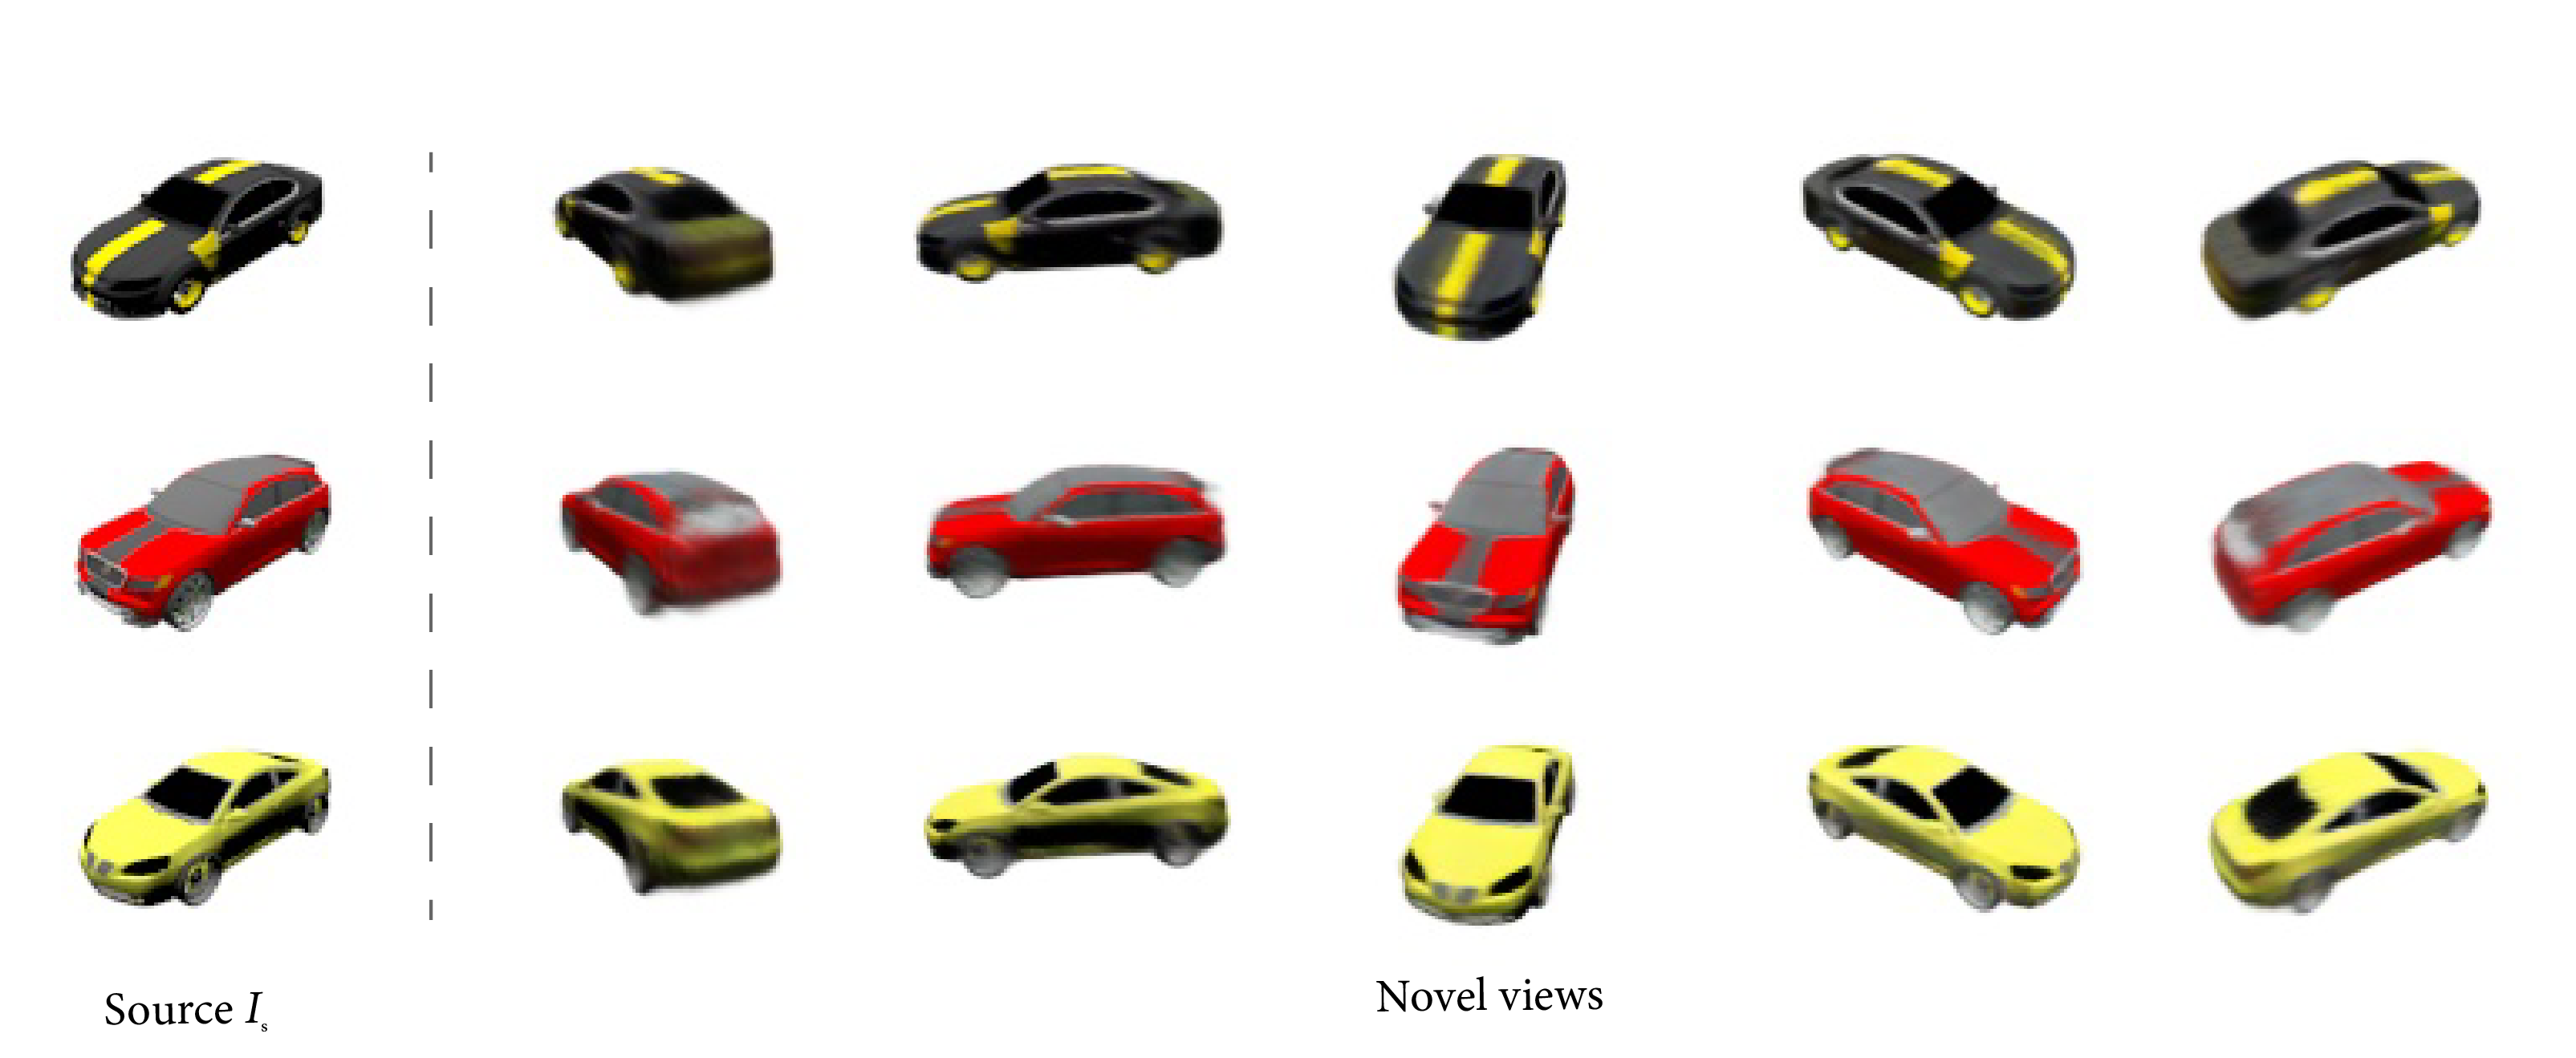
\includegraphics[width=\linewidth]{images/epinerf/supp_NVS_Cars.png}
  \caption{\textbf{Novel view synthesis.} Additional views on ShapeNet-SRN \textit{Cars} class are rendered from a broad range of viewpoints given a single source image. }
  \label{fig:supp_NVScars}
  \end{center}
\end{figure}


\begin{figure}[htp!]
    \begin{center}
  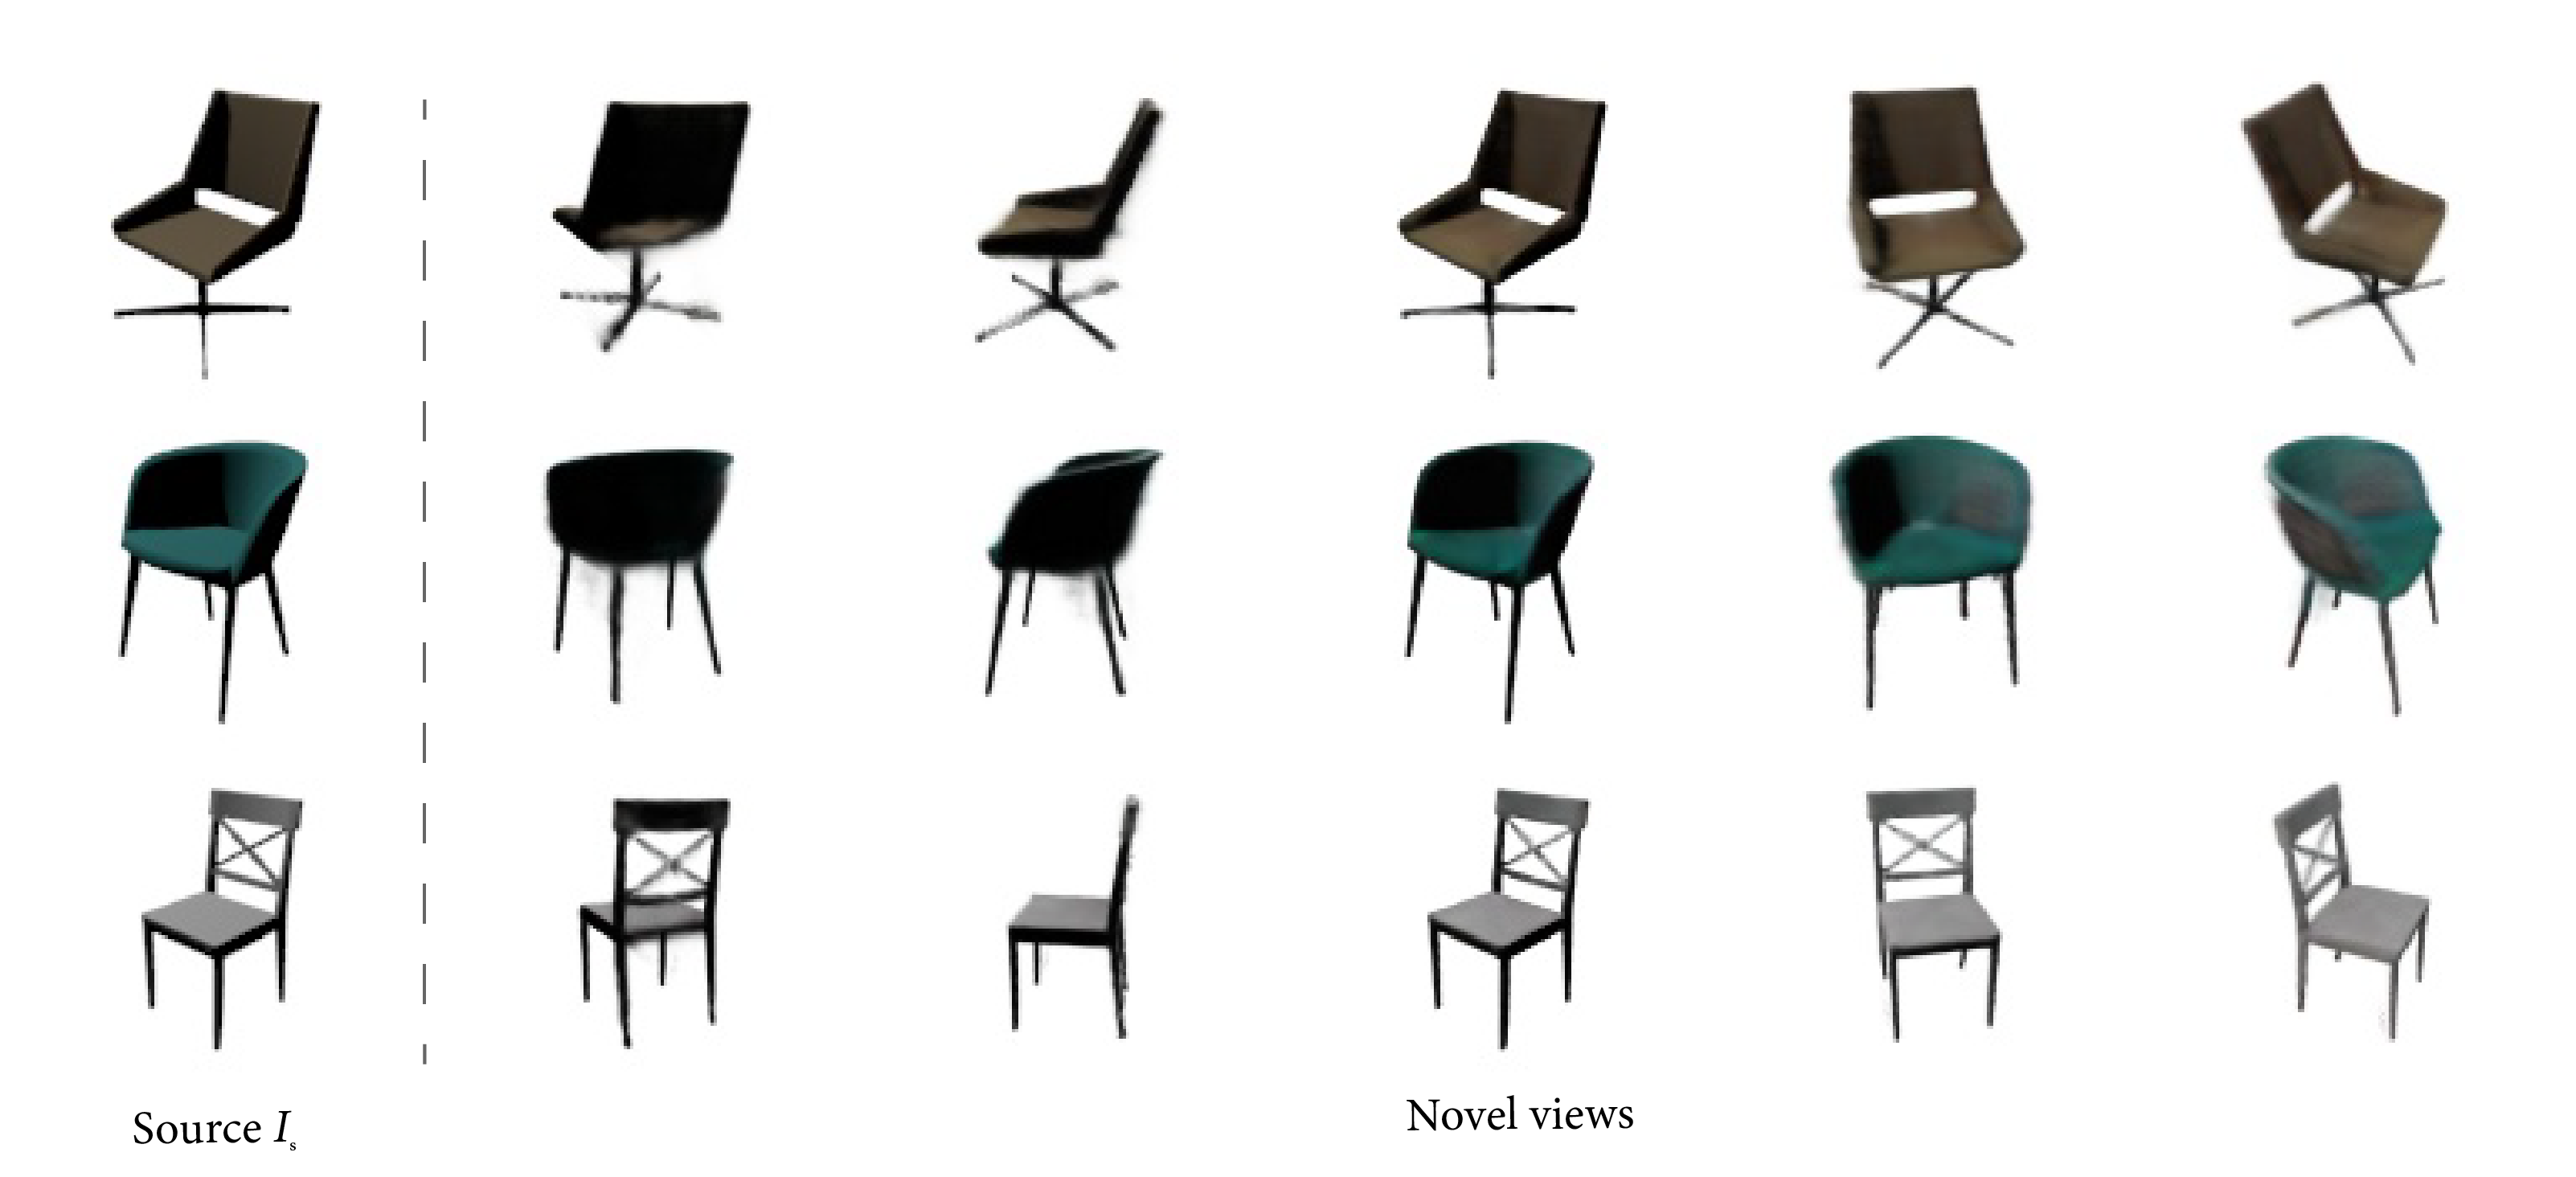
\includegraphics[width=\linewidth]{images/epinerf/supp_NVS_Chairs.png}
  \caption{\textbf{Novel view synthesis.} Additional views on ShapeNet-SRN \textit{Chairs} class are rendered from a broad range of viewpoints given a single source image. }
  \label{fig:supp_NVSchairs}
  \end{center}
\end{figure}

Figures \ref{fig:supp_cars} and \ref{fig:supp_chairs} depict additional side-by-side renderings against state-of-the-art methods. As mentioned in the main paper, EpiNeRF, through its consideration for target-aligned features from $\Psi$, managed to better handle occlusions or unseen parts in view generation compared to current state-of-the-art methods. Armrests and door paintings are rendered with sharper details. EpiNeRF achieves these NVS performances without requiring a large pool of GPUs for training, unlike the VisionNeRF \cite{lin2023vision} approach.

\begin{figure*}[htp!]
    \begin{center}
  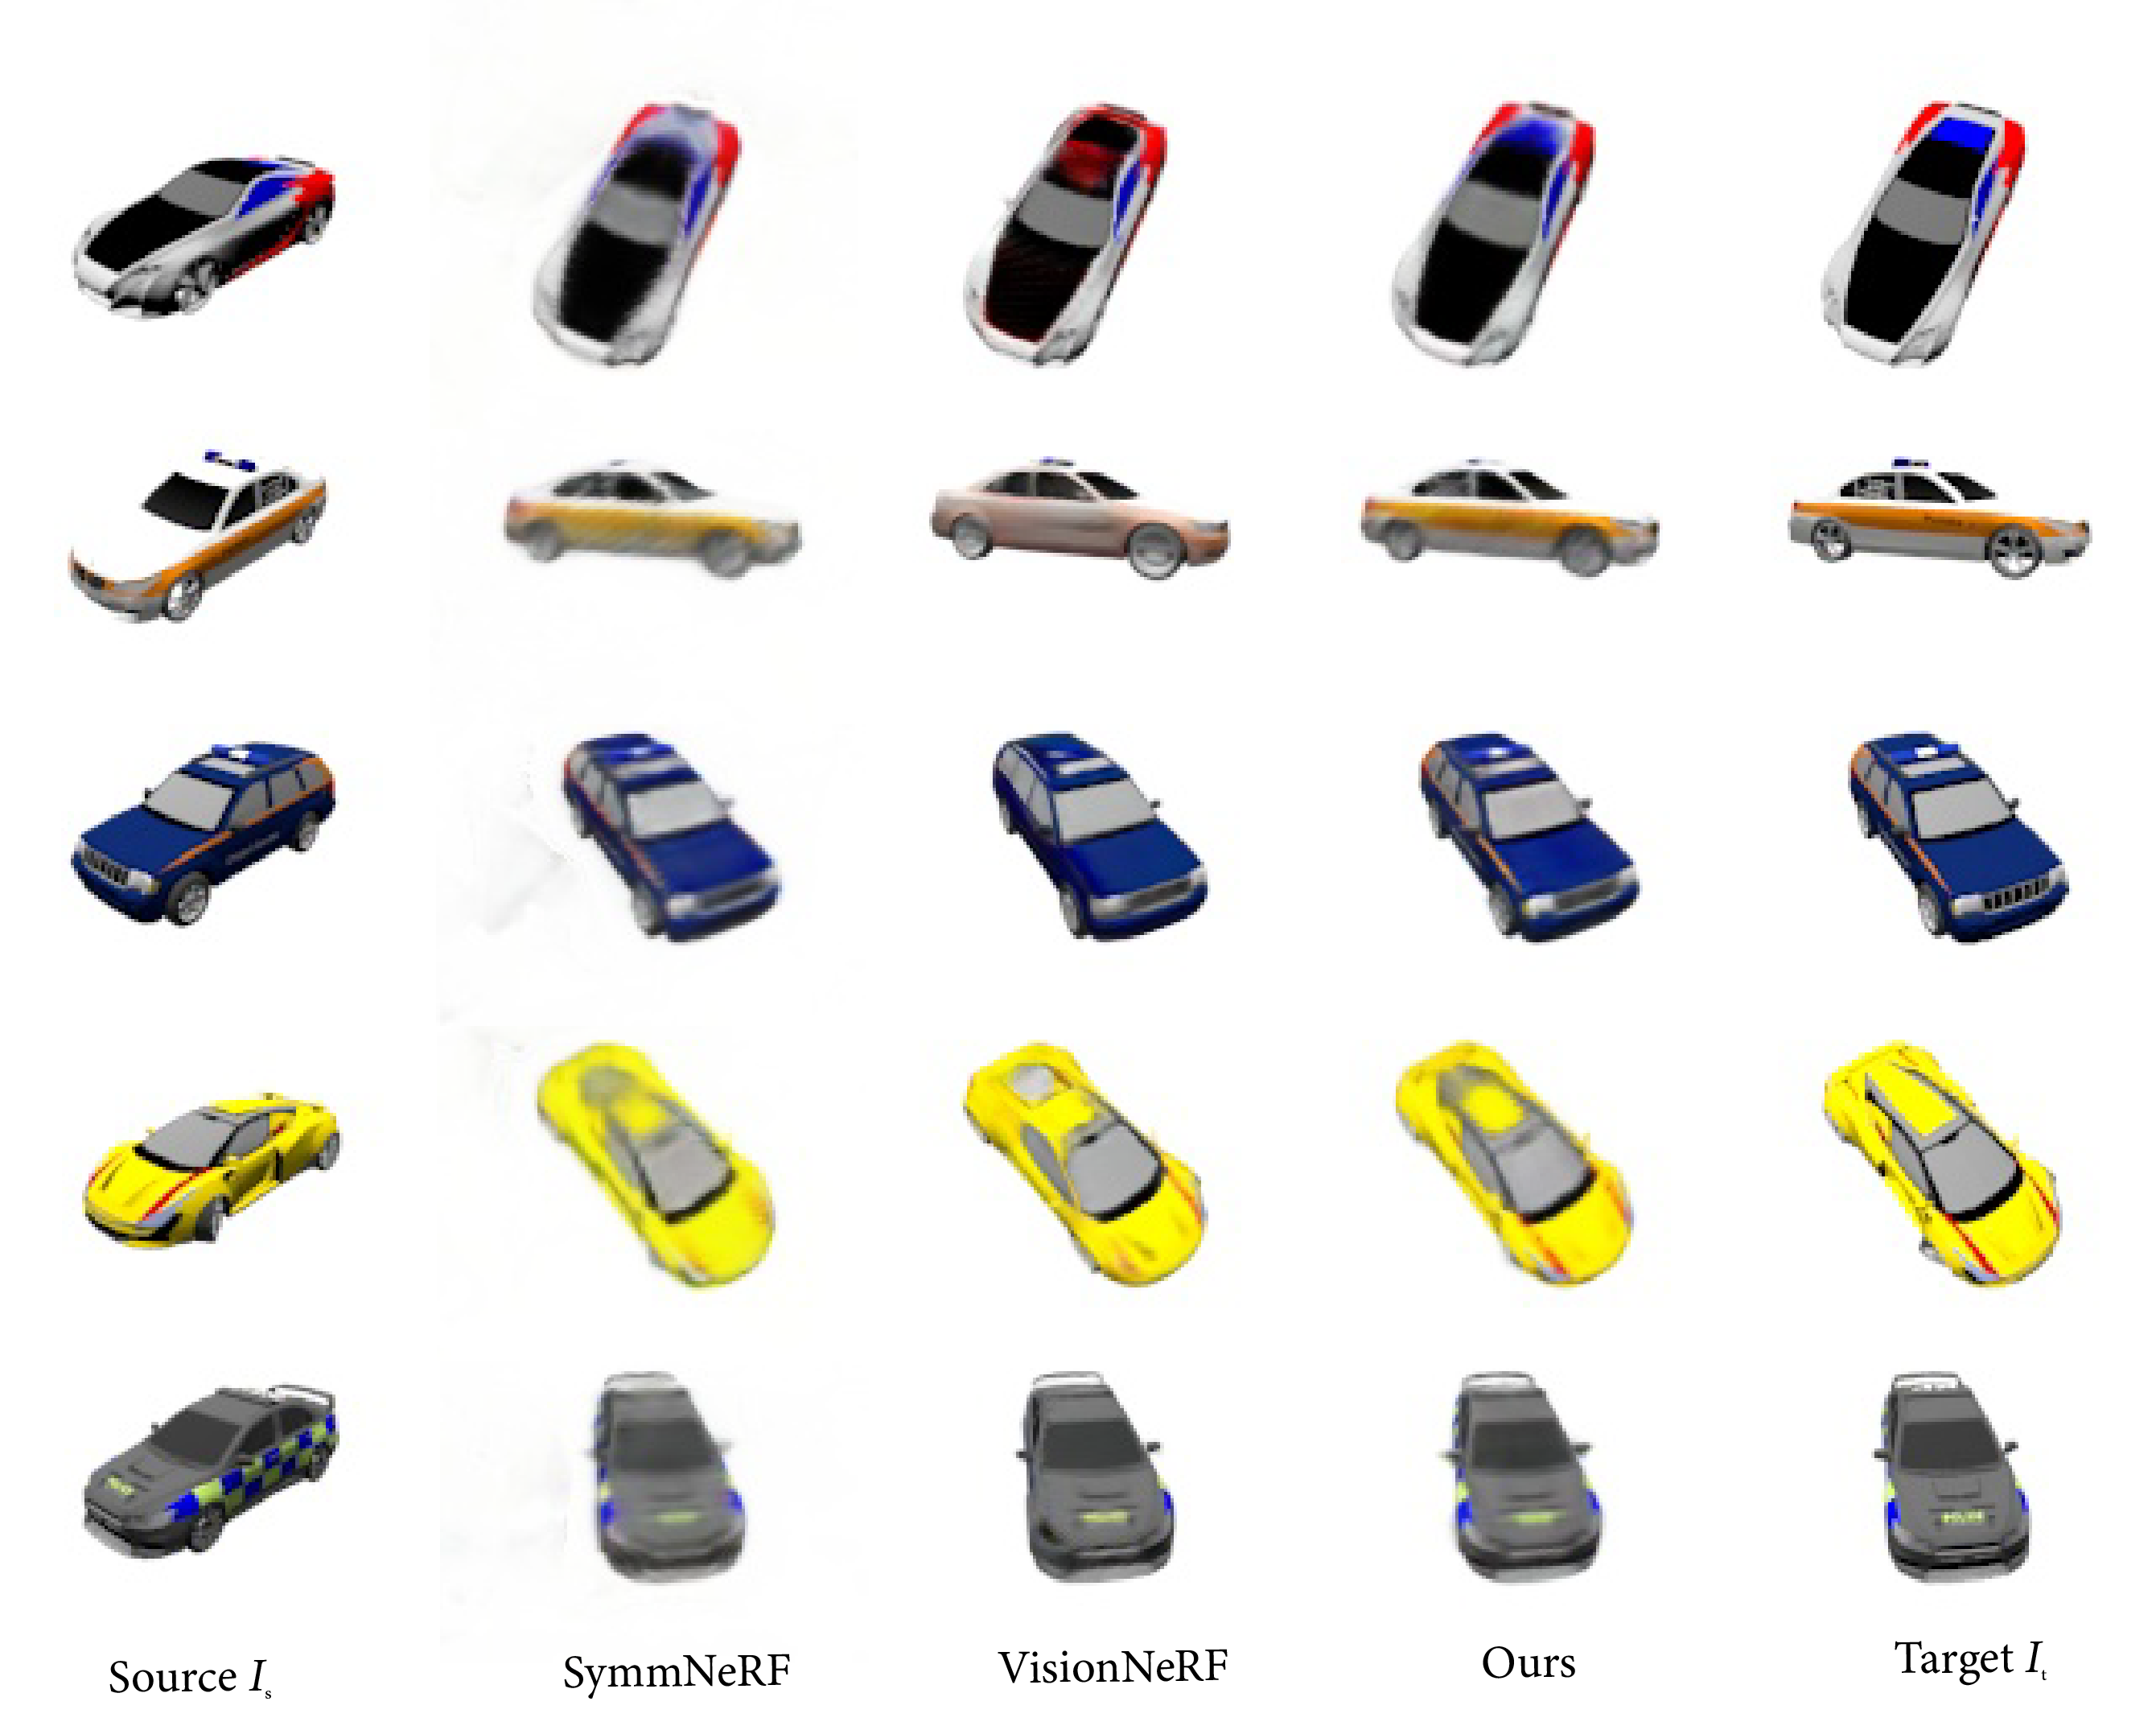
\includegraphics[width=\linewidth]{images/epinerf/supp_Cars_additional_inference.png}
  \caption{\textbf{Novel view synthesis on the ShapeNet category-specific} \textit{Cars. }EpiNeRF generates sharper views than SymmNeRF while preserving the symmetry aspects that VisionNeRF failed to maintain.}
  \label{fig:supp_cars}
  \end{center}
\end{figure*}


\begin{figure*}[htp!]
    \begin{center}
  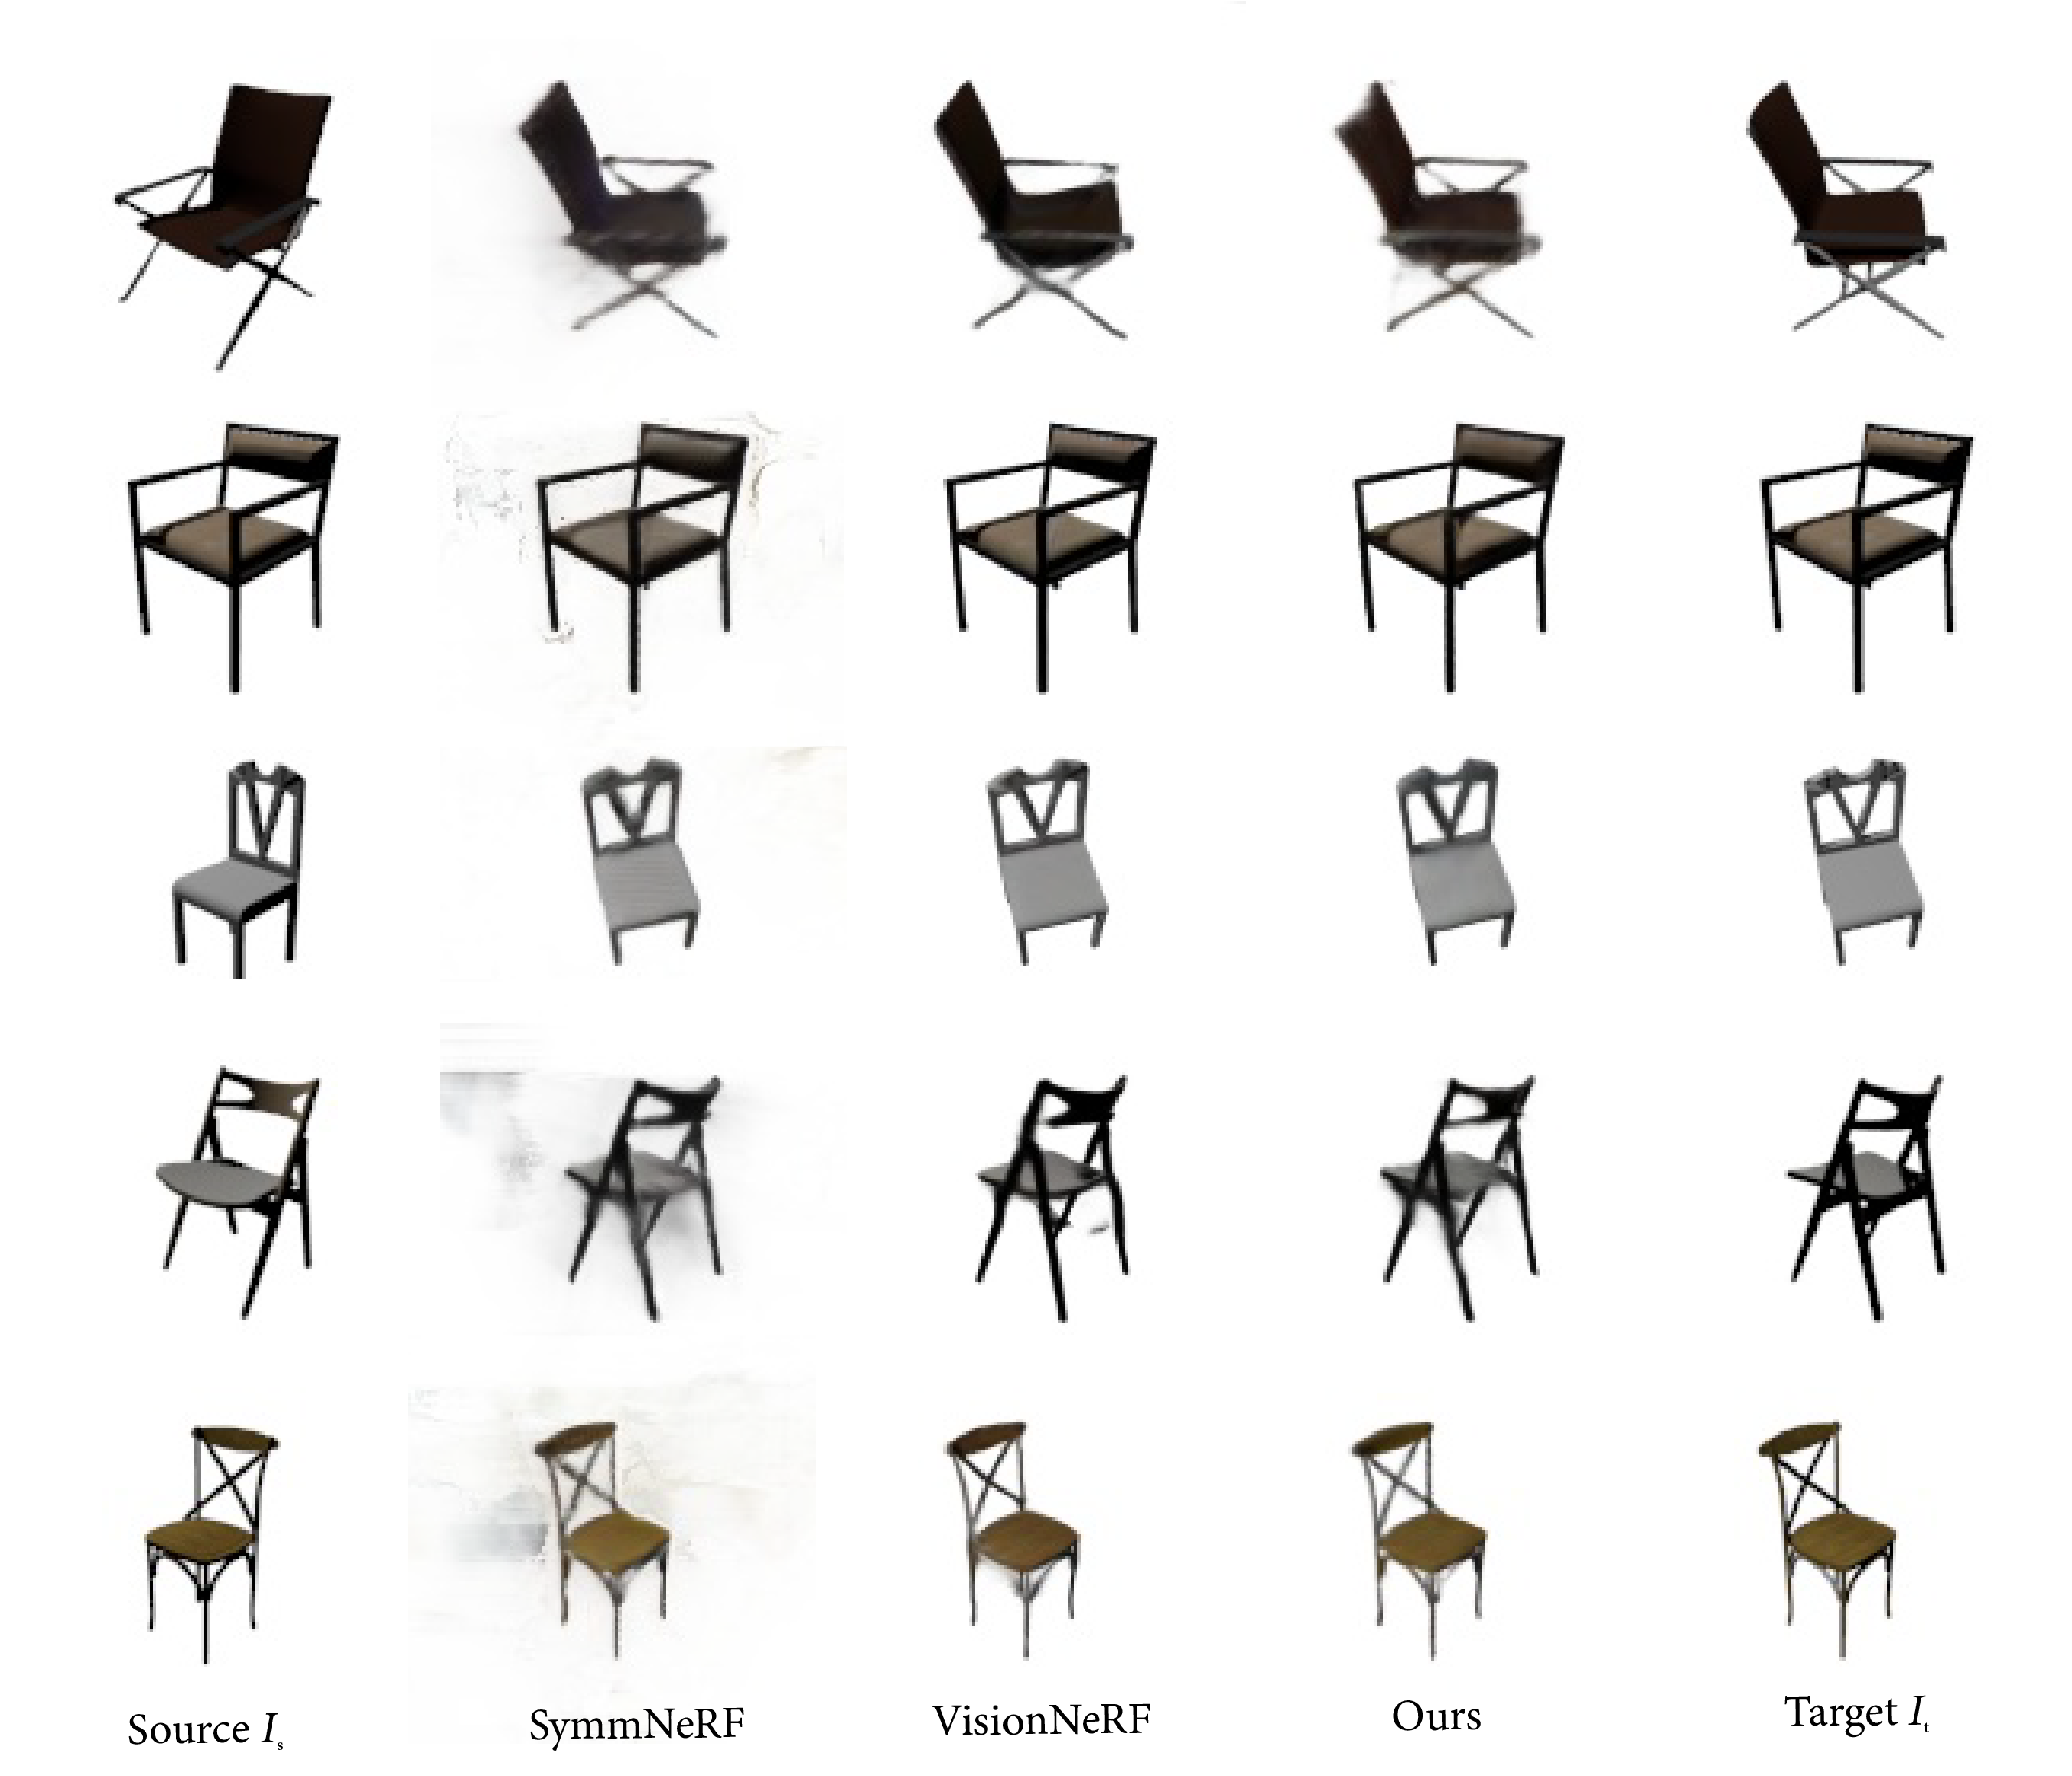
\includegraphics[width=\linewidth]{images/epinerf/supp_Chairs_additional_inference.png}
  \caption{\textbf{Novel view synthesis on the ShapeNet category-specific} \textit{Chairs. }EpiNeRF generates sharper views than SymmNeRF while preserving the symmetry aspects that VisionNeRF failed to maintain.}
  \label{fig:supp_chairs}
  \end{center}
\end{figure*}

\chapter{Additional ressource about 3D Gaussian Splatting for CarCutter}

We present in this last annex some additional information regarding the Chapter ~\ref{chapter:gausssplat}. 

\section{Gaussian primitives transformation}
\label{appendix:cov}
Let's first get into the equation \ref{eq:gs-3dcov-transfrom} presented in Chapter \ref{chapter:gausssplat}, to transform the 3D covariance $\Sigma^{(k)}_{3D}$ from world to camera coordinate system.

Given the linear transformation $R$ and the translation $t$, one can thus express any point $p$ in the world coordinate into its camera coordinate counter part through $p' = R\times p + t$. We thus also have the revert operation with: $p = R^{-1}\times (p' - t)$. 

The 3D gaussian primitive $\mathcal{G}_{k}$: 

\begin{equation}
    \mathcal{G}_{k}(p) = \exp \left(-\frac{1}{2}(p-\mu^{(k)}_{3D})^{T}(\Sigma^{(k)}_{3D})^{-1}(p-\mu^{(k)}_{3D})\right)
  \end{equation}
  
is thus transformed through: 
\begin{equation}
    \begin{aligned}
    \mathcal{G}_{k}(p) &= \exp \left( -\frac{1}{2} \{R^{-1}(p'-t) - R^{-1}(\mu^{(k)}_{cc} -t)\}^{T} (\Sigma^{(k)}_{3D})^{-1}\{R^{-1}(p'-t) - R^{-1}(\mu^{(k)}_{cc} -t)\}  \right) \\
    &= \exp \left( -\frac{1}{2}\{ R^{-1}(p'-\mu^{(k)}_{cc})\}^{T}(\Sigma^{(k)}_{3D})^{-1})\{ R^{-1}(p'-\mu^{(k)}_{cc})\} \right) \\
    &= \exp \left( -\frac{1}{2}(p'-\mu^{(k)}_{cc})^{T}R\times(\Sigma^{(k)}_{3D})^{-1}\times R^{-1}(p'-\mu^{(k)}_{cc})\right) \\
    &= \exp \left( -\frac{1}{2}(p'-\mu^{(k)}_{cc})^{T}(\Sigma^{(k)}_{3D})^{-1}(p'-\mu^{(k)}_{cc})\right) \\
    \end{aligned}
\end{equation}

with thus $\Sigma^{(k)}_{3D} = R\times \Sigma^{(k)}_{3D}\times R^{-1}$. 


Considering the affine approximation of $\phi$, we thus have from Equation \eqref{eq:affine_transform}: 

\begin{equation}
  \phi(p') - \phi(\mu_{cc}) \approx J(p' - \mu_{cc})
\end{equation}

and the primitive $\mathcal{G}_{k}$ is expressed in the ray space as: 

\begin{equation}
  \begin{aligned}
\mathcal{G}_{k}(\phi(p')) &= \exp \left( -\frac{1}{2}(\phi(p')-\phi(\mu^{(k)}_{cc}))^{T}(\Sigma^{(k)}_{3D})^{-1}(\phi(p')-\phi(mu^{(k)}_{cc}))\right)\\
                        &= \exp \left( -\frac{1}{2}(J_{k}(p'-\mu^{(k)}_{cc}))^{T}(\Sigma^{(k)}_{3D})^{-1}(J_{k}(p'-mu^{(k)}_{cc}))\right) \\
                        &= \exp \left( -\frac{1}{2}(p'-\mu^{(k)}_{cc})^{T}J_{k}^{T}(\Sigma^{(k)}_{3D})^{-1}J_{k}(p'-mu^{(k)}_{cc})\right)\\
                        &= \exp \left( -\frac{1}{2}(p'-\mu^{(k)}_{cc})^{T}(J_{k}\Sigma^{(k)}_{3D}J_{k}^{T})^{-1}(p'-mu^{(k)}_{cc})\right)
  \end{aligned}
\end{equation}

As explained in \citep{zwicker2001ewa}, one can drop the thrid row and column of  $ \Sigma^{(k)}_{ic}$ to get a 2D covariance matrix, named $\Sigma^{(k)}_{2D}$. Applying a projective transformation to any 3D gaussian primitive $\mathcal{G}_{k}$ lead to the scaled 2D gaussian primitive, termed $g_{k}$: 

\begin{equation}
    g_{k}(x) = \exp(-\frac{1}{2}(x-\mu^{(k)}_{2D})^{T}(\Sigma^{(k)}_{2D})^{-1}(p-\mu^{(k)}_{2D}))
  \end{equation}

with $\mu^{(k)}_{2D}= \phi(\mu_{cc}^{k})$ and $\Sigma^{(k)}_{2D}= J\Sigma^{(k)}_{cc}J^{T}$ the 2D mean and $2\times2$ covariance matric of $ g_{k}$. 


\section{Spherical Harmonics: How color is made view-dependent ?}
\label{appendix:gs-sh}

A gaussian primitive $\mathcal{G}_{k}$ do not store the color information through an RGB value. Authors from 3D-\ac{GS} indeed rather made color view-dependent by relying on \ac{SH} functions. 

The normalized viewing direction $\mathbf{d}$ we looking at can thus be expressed in spherical coordinates through the tuple of angles $(\theta,\phi)$. \ac{SH} functions are defined on sphere surface with \textit{l} of bands and $-l \leq  m \leq m$ elementary functions $Y_{l}^{m}$ within each band.

\begin{equation}
    Y_{l}^{m}(\theta,\phi) = \frac{(-1)^{l}}{2^{l}l!} \times \sqrt{\frac{(2l+1)(l+m)!}{4\pi(l-m)!}}e^{im\phi}(sin(\theta))^{-m}\frac{d^{l-m}sin(\theta)^{2l}}{d(cos(\theta)^{l-m})}
\end{equation}

\ac{GS} usually considers 4 bands of \ac{SH}, and consider the view-dependent color $c$: 

\begin{equation}
    c(\mathbf{d}) = \sum_{l=0}^{3}\sum_{m=-l}^{m=l}k_{l}^{m}Y_{l}^{m}(\mathbf{d})
\end{equation}

while the $k_{l}^{m}$ are the \ac{SH}-coefficient that needs to be learned during training per gaussian primitives. 


\end{equation}

\section{Undetermined positional gradient signs in the ADC}
\label{appendix:sign-gradient}

As mentioned in Section ~\ref{gs:pixgs-adc}, the per-pixel gradient $\frac{\partial L_{j}}{\partial \mu^{k}_{ndc,x}}$ is expressed as a sum of product terms that might have different signs. 

We thus already expressed such a per-pixel gradient for the x-axis as: 

\begin{equation}
    \label{eq:perpix-grad}
    \frac{\partial L_{j}}{\partial \mu^{k}_{ndc,x}} = \sum \limits_{l=1}^{3} \frac{\partial L_{j}}{\partial c_{l}^{j}}\times \frac{\partial c_{l}^{j}}{\partial \alpha_{k}^{j}} \times \frac{\alpha_{k}^{j}}{\partial \mu^{k}_{ndc,x} }
    \end{equation}

\begin{itemize}
    
    \item \textbf{First term} $\frac{\partial L_{j}}{\partial c_{l}^{j}}$ 
This partial derivative is rather straightforward as $\partial L_{j}$ define the $L_{1}$ loss function between the rendered pixel color and the ground truth one. This first term is thus either set to $+1$ or $-1$ and its sign is undertermined as soon as the difference between predicted and ground truth color can either be positive or negative. 

    \item \textbf{Second term} $\frac{\partial c_{l}^{j}}{\partial \alpha_{k}^{j}}$ 
The second term has to be developed to fully grasp why it also exists a sign ambiguity in its expression. Accounting on the expression of the rendered color in Equation \eqref{eq:gs-alpha-blending}, such partial derivative can thus be derived as follow. We drop here both the channel  \textit{l} as well as the pixel \textit{j} indexing for sake of clarity.  

\begin{equation}
    \frac{\partial c_{l}^{j}}{\partial \alpha_{k}} = c_{k} \times \prod \limits_{p=1}^{k-1}(1 - \alpha_{p}) - \sum \limits_{q=k+1}^{K} c_{q}\alpha_{q}\prod \limits_{p=1,p\neq q}^{q-1}(1 - \alpha_{p})
\end{equation}
Whearas both term are positives, their difference made such a term undetermined regarding its sign. 

    \item \textbf{Third term} $\frac{\partial \alpha_{k}^{j}}{\partial \mu^{k}_{ndc,x}}$ 
This last term can directly be derived from Equation \eqref{eq:gs-alpha-def}. The aformentioned equation can be fully developped through: 
\begin{equation}
    \alpha_{k}^j(pix) =o_{k} \times g_{k}(pix) =  o_{k} \times \exp \left( -\frac{1}{2} \mathbf{d}^T \left( \Sigma_{2D}^{(k),j} \right)^{-1} \mathbf{d} \right),  
\end{equation}
where $\mathbf{d} = \begin{pmatrix}
    p_x - \mu_{2D,x}^{(k),j} \\
    p_y - \mu_{2D,y}^{(k),j}
\end{pmatrix}$ and $pix=\left( p_{x},p_{y}\right)^{T}$ 

We thus get for the last partial derivative: 
\begin{equation}
    \frac{\partial \alpha_{k}^{j}}{\partial \mu^{(k)}_{ndc,x}} =  o_{k} \times \frac{\partial g_{k}}{\partial \mu^{k}_{ndc,x}} = o_{k} \times g_{k} \times ((\Sigma_{2D}^{(k),j})^{-1}\mathbf{d})_{x}
\end{equation}
The sign of this third and last term thus directly depends on the sign of $\mathbf{d}_{x} = p_x - \mu_{2D,x}^{(k),j}$, which is undetermined. 

\end{itemize}






